\documentclass[11pt]{book}
\usepackage{geometry}
\usepackage{palatino}
\usepackage[all]{xy}
\geometry{letterpaper}
\usepackage{amsthm,amssymb,amsmath,graphicx}
\usepackage{mathrsfs,amscd}
\usepackage{multirow}
\newtheorem{theorem}{Theorem}[section]
\newtheorem{conjecture}[theorem]{Conjecture}
\newtheorem{claim}[theorem]{Claim}
\newtheorem{corollary}[theorem]{Corollary}
\newtheorem{lemma}[theorem]{Lemma}
\newtheorem{proposition}[theorem]{Proposition}
\newtheorem{example}[theorem]{Example}
\newtheorem{exercise}[theorem]{Exercise}
\newtheorem{remark}[theorem]{Remark}
\newtheorem{algorithm}[theorem]{Algorithm}
\newtheorem{definition}[theorem]{Definition}
\newcommand{\bb}[1]{\mathbb{#1}}
\newcommand{\mc}[1]{\mathcal{#1}}
\newcommand{\mf}[1]{\mathfrak{#1}}
\linespread{1.1}
\title{MATH 5145 - Lie Groups and Lie Algebras}
\date{}
\begin{document}
\maketitle
\tableofcontents

\newpage
\chapter{Differentiable Manifolds}
\section{Basic Definition}
Let $M \subset \bb{R}^m$ be equipped with the usual (Euclidean) topology. Then $M$ is a \textbf{topological manifold} of dimension $n$ if:\\

For all $p \in M$, there exists open set $U$ containing $p$ so that we have a homeomorphism
$$\phi: U \to \tilde{U} \subset \bb{R}^n$$
where $\tilde{U}$ is open in $\bb{R}^n$. The map $\phi$ is called the \textbf{local coordinates} of $U$.
\begin{example}
Let
$$M  = S^2 := \left\{ x = (x_1, x_2, x_3)\ \Big|\ \sum_i x_i^2 = 1 \right\} \subset \bb{R}^3$$
We need to give local coordinates for every point $p \in S^2$. There are many such options, for example define open sets
$$U_i^{\pm} := \left\{ x \in S^2\ \Big|\ x_i > 0 \right\}$$
Then every $p \in S^2$ must lie in at least one of the $U_1^{\pm}, U_2^{\pm}, U_3^{\pm}$.
and define the local coordinates
$$\phi_i^{\pm} : U_i^{\pm} \to \left\{(a,b) \in \bb{R}^2\ \Big|\ a^2 + b^2 < 1 \right\}$$
by omitting the $x_i$ coordinates.\\
Check that $\phi_i^{\pm}$ is:\\
1) one-one and onto\\
2) differentiable\\
and its inverse is also differentiable (exercise). Therefore, all the local coordinates are homeomorphisms, and $S^2$ is a topological manifold.
\end{example}
\begin{exercise}
Fill in the details in the above Example.
\end{exercise}
In order to make a topological manifold differentiable, we need the following:
\begin{definition}
An \textbf{atlas} of a topological manifold $M$ is a collection of $\left\{(U_{\alpha}, \phi_{\alpha})\right\}$ that covers $M$.\\
Suppose $(U,\phi)$ and $(V,\phi)$ are two homeomorphisms in an atlas of $M$ such that $U \cap V$ is non-empty. The \textbf{transition map} is
$$ \phi \circ \psi^{-1} : \psi(U \cap V) \to \phi(U \cap V)$$
which is a map from an open subset of $\bb{R}^n$ to an open subset of $\bb{R}^n$.
\end{definition}
We can now define smooth manifolds:
\begin{definition} \mbox{}\\
- A \textbf{smooth atlas} of a topological manifold $M$ is an atlas so that $\phi \circ \psi^{-1}$ is smooth (infinitely differentiable, $C^{\infty}$) for all $(U,\phi)$ and $(V,\phi)$ such that $U \cap V$ is non-empty.\\
- We say that two atlas $\mc{A}, \mc{B}$ for $M$ are \textbf{equivalent} if the local charts of one are compatible with those of the other, namely, $\phi \circ \psi^{-1}$ is smooth for all $(U, \phi) \in \mc{A}$, $(V, \psi) \in \mc{B}$. \\
- A \textbf{smooth structure} on $M$ is an equivalence class $[\mc{A}]$ of smooth atlases on $M$.\\
- A \textbf{smooth manifold} is a 2-tuple $(M,[\mathcal{A}])$ where $M$ is a topological manifold and $\mathcal{A}$ is a smooth atlas.
\end{definition}
The definition of a smooth manifold looks somewhat unintuitive - especially the notion of equivalence class of an atlas. We will see it is necessary very soon (see \ref{sub} for instance). But for now, we just need to know that if $M$ is a topological manifold with a smooth atlas $\mc{A}$, then $(M, [\mc{A}])$ is automatically a smooth manifold.\\
We state the following fact about equivalence class of atlases without proving it:
\begin{theorem}
Suppose $\mc{A}$ is a smooth atlas of a manifold $M$, and $\mc{B}$ is another atlas compatible with $\mc{A}$, then $\mc{A} \cup \mc{B}$ is also a smooth atlas of $M$.\\
Consequently, for any equivalence class of of atlases $[\mc{A}]$, there exists a unique maximal class $\mc{A}_{max} \in [\mc{A}]$.
\end{theorem}

\begin{example}\mbox{}\\
- Example 1.1 is an example of a smooth manifold.\\
- $M = \bb{R}^n$ is a smooth manifold (with atlas $(M, id: M \to \bb{R}^n)$). So is $M = \bb{C}^n \equiv \bb{R}^{2n}$.\\
- The collection of all $n \times n$ real or complex matrices $M_{n}(\bb{R})$ or $M_{n}(\bb{C})$.\\
- Any open subset $W$ of a smooth manifold $M$ gives a smooth manifold (of the same dimension). Namely, if $\left\{(U,\phi)\right\}$ is a smooth atlas of $M$, then so does $\left\{(U \cap W, \phi  \Big|_{U \cap W})\right\}$.\\
- The above realization gives us the first example of matrix Lie groups:
$$GL(n,\bb{R}) := \left\{ g \in M_{n}(\bb{R})\ \Big|\ \det(g) \neq 0 \right\} $$
Since the map $det: M_n(\bb{R}) \to \bb{R}$ is continuous, $GL(n,\bb{R}) = det^{-1}\left\{(-\infty,0)\cup(0,\infty)\right\}$ is an open set in $M_n(\bb{R})$.\\
- Other matrix Lie groups (whose smooth atlas is not obvious for now):\\
$$SL(n,\bb{R}) = \left\{ g \in GL(n,\bb{R})\ \Big|\ \det(g) = 1 \right\}$$
$$O(n,\bb{R}) = \left\{ g \in GL(n,\bb{R})\ \Big|\ g^Tg = Id \right\}$$
we will study more on them next Chapter.\\
- (Product of manifolds) If $M$ and $N$ are smooth manifolds, so is their Euclidean product $M \times N$.
\end{example}
Here is a class of manifolds we will study a lot next Chapter:
\begin{definition}\label{sub}
Let $(M,[\mc{A}])$ is a smooth manifold of dimension $n+k$. A subset $S \subset M$ is a \textbf{smooth embedded submanifold} of dimension $n$ if for each point $p \in S$, there exists $(U, \phi) \in \mc{A}_{max}$ of $M$ so that $p \in U \cap S$, and the local coordinate map
$$\phi : U \to \phi(U) \subset \bb{R}^{n+k}$$
satisfies
$$\phi(U \cap S) \subset \bb{R}^k = \left\{ (x_1, \dots, x_{n+k}) \in \bb{R}^{n+k}\ \Big|\ x_{n+1} = x_{n+2} = \dots = x_{n+k} = 0 \right\}$$
\end{definition}
\begin{example}
$S^2 \subset \bb{R}^3$ is a smooth embedded manifold of $(\bb{R}^3, [(\bb{R}^3, id)])$.\\
This is the first instance where we see the equivalence class abstraction is necessary - if we only have the atlas $id:\bb{R}^3 \to \bb{R}^3$, then $id  \Big|_{S^2} : S^2 \to \bb{R}^3$ can never satisfy Definition \ref{sub}.\\
With the flexibility of equivalence class, we can define an atlas $(U_i^{\pm}, \phi_i^{\pm}), (V, id)$ of $\bb{R}^3$ by
$$U_i^{\pm} = \left\{ (x_1, x_2, x_3) \in \bb{R}^3\ \Big|\ x_i > 0 \text{ (or } x_i< 0) \right\}, V := \left\{ (x_1, x_2, x_3) \in \bb{R}^3\ \Big|\ x_1^2 + x_2^2 + x_3^2 < 0.5 \right\}$$
$$\phi_1^{\pm}: (x_1, x_2, x_3) \mapsto (x_2, x_3, 1-x_1^2-x_2^2-x_3^2)$$
$$\phi_2^{\pm}: (x_1, x_2, x_3) \mapsto (x_1, x_3, 1-x_1^2-x_2^2-x_3^2)$$
$$\phi_3^{\pm}: (x_1, x_2, x_3) \mapsto (x_1, x_2, 1-x_1^2-x_2^2-x_3^2)$$
so that $(U_i^{\pm}, \phi_i^{\pm}), (V, id) \in \mc{A}_{max}$. And they are of the form in Definition \ref{sub}.
\end{example}
\section{Smooth Maps between Manifolds}
\begin{definition}
A map $f: M \to \bb{R}^k$ is \textbf{smooth} if for every $p \in M$, there exists open set $(U,\phi)$ containing $p$ such that
$$f \circ \phi^{-1} : \phi(U) \to \bb{R}^k$$
is smooth. Equivalently, if $(U,\phi)$ is a smooth atlas of $M$, then $f \circ \phi^{-1}$ is smooth for all $(U, \phi)$.\\
\end{definition}
Note that the above definition does not depend on the choice of local coordinates in $\mc{A}_{max}$ - indeed, two different choices of local coordinates only differs $f$ by $\phi \circ \psi^{-1}$, which is smooth by definition.\\
We write
$$C^{\infty}(M) = \left\{ f: M \to \bb{R}\ \text{is a smooth map}\right\}$$
Similarly, a map $f: M \to N$ is smooth if for any local coordinates $(U,\phi)$ and $(V,\psi)$ of $M$ and $N$ respectively,
$\psi \circ f \circ \phi^{-1}$ is smooth in the suitable domain.

\begin{example}
$\iota: S^n \to \bb{R}^{n+1}$ is smooth. For any $U_i^{\pm}$, the map is given by
$$(u_1, \dots, u_n) \stackrel{\iota \circ \phi_i^{-1}}{\longrightarrow} (u_1, \dots, u_{i-1}, \pm\sqrt{1- \sum_k u_k^2}, u_{i+1}, \dots, u_n)$$
\end{example}
Here is the definition of Lie group:
\begin{definition}
A \textbf{Lie group} is a smooth manifold $G$ so that it has a group structure, and the multiplication and inverse map
$$m: G \times G \to G\ ;\ i: G \to G$$
$$m(g,h) = gh\ ;\ i(g) = g^{-1}$$
are both smooth maps.
\end{definition}
For example, $GL(n,\bb{R})$ is a Lie group - write the coordinates of $G \times G$ as $(x_{ij}, y_{ij})$, then $m(g,h) = (m_{11}(gh), m_{12}(gh), \dots, m_{nn}(gh))$ given by
$$m_{kl}(x_{ij}, y_{ij}) = x_{k1}y_{1l} + x_{k2}y_{2l} + \dots + x_{kn}y_{nl}$$
for each $1 \leq k,l \leq n$. Similarly, the inverse map is smooth using the formula $A^{-1} = \frac{1}{\\det(A)}adj(A)$.
Since multiplication and inverse are the same for other matrix groups $SL(n,\bb{R})$, $SO(n,\bb{R})$, they automatically become Lie groups once we have shown they are embedded submanifolds of $GL(n,\bb{R})$.
\section{Tangent Space of a Manifold} In smooth manifolds, we need to use an abstract way to define tangent vectors. Let's look at the case of $M = \bb{R}^n$:
Let $a \in M$, then the tangent space at $a$, which we denote as $T_aM$ is just the space $\bb{R}^n$. We will instead look at the directional derivative at $a$ rather than the tangent vector as follows:
$$tangent\ vector\ v_a \in T_a\bb{R}^n \stackrel{1:1}{\longleftrightarrow}\ directional\ derivative\ D_{v_a}$$
where $D_{v_a}: C^{\infty}(\bb{R}^n) \to \bb{R}$ given by
$$D_{v_a}(f) := \frac{d}{dt}f(a+tv)  \Big|_{t = 0}$$
suppose the local coordinates is given by $x_1, x_2, \dots, x_n$, then
$$D_{v_a}(f) = \frac{d}{dt}f(a+tv)  \Big|_{t = 0} = \frac{d}{dt}f(x_1(t), \dots, x_n(t))  \Big|_{t = 0}$$
with $x_i(t) = a_i + tv_i$, so chain rule gives
$$D_{v_a}(f) = \frac{d}{dt}f(a+tv)  \Big|_{t = 0} = \sum_i \frac{dx_i}{dt}\frac{\partial f}{\partial x_i}(a) = \sum_i v_i\frac{\partial f}{\partial x_i}(a)$$

For general manifold $M$:
\begin{definition}
A \textbf{tangent vector} at $p \in M$ is a linear map
$$X_p : C^{\infty}(M) \to \bb{R}$$
satisfying the Leibniz rule, i.e.
$$X_p(fg) = f(p)X_p(g) +g(p)X_p(f)$$
the collection of all such maps is the \textbf{tangent space} $T_pM$.
\end{definition}
For example,
$$T_a(\bb{R}^n) = \mathrm{Span}\left\{ \frac{\partial }{\partial x_1}  \Big|_a, \frac{\partial }{\partial x_2}  \Big|_a, \dots, \frac{\partial}{\partial x_n}  \Big|_a \right\}$$
Suppose $(U,\phi: U \to \tilde{U} = \mathrm{Span}\left\{x_1, \dots, x_n\right\})$ is a local coordinate of $M$ with $p \in U \subset M$, then we can express the tangent vector locally by
$$a_1\frac{\partial }{\partial x_1}  \Big|_p +  \dots +  a_n \frac{\partial }{\partial x_n}  \Big|_p$$
Given a map of smooth manifolds, we can also map tangent vectors by the following:
\begin{definition}
Let $M$ and $N$ be smooth manifolds, and $F: M \to N$ is a smooth map. The \textbf{push-forward} $F_*$ is defined by
$$F_*: T_pM \to T_{F(p)}N$$
$$X \mapsto F_*X$$
where $F_*X(f) := X(f \circ F)$ for any $f \in C^{\infty}(N)$.
\end{definition}
Obviously, if $F_1 : M_1 \to M_2$ and $F_2: M_2 \to M_3$ are smooth maps, then $(F_2 \circ F_1)_* = (F_2)_* \circ (F_1)_*$.
\begin{example}
Let $F: M \to \bb{R}^k$, and $X_p := \frac{\partial }{\partial x_1}  \Big|_p \in T_pM$. What is $F_*(\frac{\partial }{\partial x_1}  \Big|_p)$?\\
For $f(y_1, \dots, y_k) \in C^{\infty}(\bb{R}^k)$,
\begin{align*}
F_*(\frac{\partial }{\partial x_1}  \Big|_p)(f) &= \frac{\partial }{\partial x_1}  \Big|_p(f \circ F) \\
&= \sum_j \frac{\partial f}{\partial y_j}(F(p)) \frac{\partial F_j}{\partial x_1}(p)\\
&= \sum_j \frac{\partial F_j}{\partial x_1}(p)\frac{\partial f}{\partial y_j}(F(p))
\end{align*}
therefore,
$$F_*(\frac{\partial }{\partial x_1}  \Big|_p) = \sum_j \frac{\partial F_j}{\partial x_1}(p)\frac{\partial }{\partial y_j}  \Big|_{F(p)}$$
\end{example}
\begin{exercise}
Let $i: S^2 \to \bb{R}^3$ be as in Example 1.9. Compute $i_*(\frac{\partial }{\partial u_1}  \Big|_{p = (\frac{1}{\sqrt{3}},\frac{1}{\sqrt{3}},\frac{1}{\sqrt{3}})})$
\end{exercise}

\section{Imbedded Submanifold}
There is another kind of submanifold we are interested in, which only involves studying the tangent space:
\begin{definition}
Let $M$ be a smooth manifold. A subset $S$ of $M$ is called an \textbf{imbedded submanifold} if $S$ is itself a smooth manifold (the topology of $S$ may not be the subset topology of $M$) and the inclusion map $i: S \hookrightarrow M$ has the property that
$$i_* : T_s(S) \to T_s(M)$$
is injective for all $s \in S$.
\end{definition}
We can show that all embedded submanifolds are imbedded submanifolds as follows: Suppose $f: S \to M$ be a smooth embedded submanifold, consider $f_*: T_s(S) \to T_s(M)$. In terms of local coordinates
$$T_s(M) = \mathrm{Span}\left\{ \frac{\partial}{\partial x_1}  \Big|_s, \frac{\partial}{\partial x_2}  \Big|_s, \dots, \frac{\partial}{\partial x_{n+k}}  \Big|_s\right\}$$
and
$$T_s(S) = \mathrm{Span}\left\{ \frac{\partial}{\partial x_1}  \Big|_s, \frac{\partial}{\partial x_2}  \Big|_s, \dots, \frac{\partial}{\partial x_{n}}  \Big|_s\right\}$$

However, \textbf{not all imbedded submanifolds are embedded submanifolds}.

\section{Vector Field}
Roughly speaking, a \textbf{vector field} on a smooth manifold $M$ is a collection of tangent vectors at different points $p \in M$, i.e.
$$X: p \in M \mapsto X_p \in T_pM$$
a smooth vector field is a vector field that changes smoothly along $p \in M$. since we do not define tangent bundle and smooth sections here we will stick with this intuition of vector bundles in this section. In local coordinates, a smooth vector bundle looks like
$$X_p = \sum_k a_k(p) \frac{\partial}{\partial x_k}  \Big|_p$$
where $a_k(p) \in C^{\infty}(U)$.\\
There is another way to look at vector fields - suppose $X$ is a vector field on a manifold $M$, and $f \in C^{\infty}(M)$. Then we can define the function $Xf \in C^{\infty}(M)$ by
$$Xf(p) := X_p(f)$$
So we have defined a map $X : C^{\infty}(M) \to C^{\infty}(M)$ given by $X(f) := Xf$. Such map has the Leibniz property, namely
$$X(fg) = X(f)g + fX(g)$$
in fact, it can be shown that every $\alpha: C^{\infty}(M) \to C^{\infty}(M)$ having the Leibniz property can be realized as a vector field.
\section{Lie bracket on Vector Fields}
Given two vector fields $V$ and $W$ on a manifold $M$, define the \textbf{Lie bracket} $[V,W]$ to be the vector field
$$[V,W]_p(f) = V_p (Wf) - W_p(Vf)$$
(check that it satisfies the Leibniz rule)\\
Here are some properties of the Lie bracket:
\begin{proposition}\label{liebracket} \mbox{}\\
An algebra $A$ over real (or complex) numbers is called a \textbf{real (or complex) Lie algebra} if there is a map $[,]: A \times A \to A$ satisfying the following properties:\\
- (bi-linearity) For all $a, b \in \bb{R}$ (or $\bb{C}$), $[aX+bY, Z] = a[X,Z] + b[Y,Z]$ and $[X,aY+bZ] = a[X,Z]+b[Y,Z]$.\\
- (skew-symmetry) $[X,Y] = -[Y,X]$.\\
- (Jacobi identity) $[X,[Y,Z]]+[Y,[Z,X]]+[Z,[X,Y]] = 0$.\\

\noindent Let $\mc{X}(M)$ be the collection of smooth vector fields on a manifold $M$. Then $\mc{X}(M)$ with the structure of the Lie bracket defined above is a real Lie algebra.
\end{proposition}
We define the Lie algebra of a Lie group by the following:
\begin{definition}
Let $G$ be a Lie group. Then the \textbf{Lie algebra} of $G$, $Lie(G)$ is the collection of all left-invariant vector fields on $G$. Equivalently, suppose $X_I$ is any tangent vector in $T_IG$, then
$$Lie(G) = \left\{ X\ \Big|\ X_g:=(L_g)_*(X_I),\ X_I \in T_I(G) \right\}$$
In particular, $Lie(G)$ satisfies the properties of Proposition \ref{liebracket}.
\end{definition}
\begin{example} \label{vfgl}
Let $G = GL(n,\bb{R})$ and compute the Lie bracket of $Lie(G)$. First of all, we need to know $T_I(G)$. Since $G$ is an open submanifold of $M_n(\bb{R})$,
$$T_I(G) = \left\{ A_{ij}\frac{\partial}{\partial x_{ij}}  \Big|_I\ \Big|\ A_{ij} \in \bb{R} \right\}\ \stackrel{1:1}{\longleftrightarrow}\ A = (A_{ij}) \in M_n(\bb{R})$$
and all $Lie(G)$ are of the form $(L_g)_*(\sum_{i,j} A_{ij}\frac{\partial}{\partial x_{ij}}  \Big|_I)$ for any matrix $A \in M_n(\bb{R})$. We write $\tilde{A}$ be its corresponding vector field, i.e.
$$\tilde{A}_g := {L_g}_*(\sum_{i,j} A_{ij}\frac{\partial}{\partial x_{ij}}  \Big|_I) = \sum_{i,j}(gA)_{ij}\frac{\partial}{\partial x_{ij}}  \Big|_g$$
(Exercise: Check the last equality holds). Now
\begin{align*}
[\tilde{A},\tilde{B}]_I(f) &= [\sum_{i,j}A_{ij}\frac{\partial}{\partial x_{ij}}, \sum_{p,q}B_{pq}\frac{\partial}{\partial x_{pq}}]_I(f)\\
 &= \sum_{i,j}A_{ij}\frac{\partial}{\partial x_{ij}}  \Big|_I (\tilde{B}f) -  \sum_{p,q}B_{pq}\frac{\partial}{\partial x_{pq}}  \Big|_I (\tilde{A}f)\\
 &= \sum_{i,j}A_{ij}\frac{\partial}{\partial x_{ij}}  \Big|_I (\sum_{p,q,r}x_{pr}B_{rq}\frac{\partial f}{\partial x_{pq}}(x)) - \sum_{p,q}B_{pq}\frac{\partial}{\partial x_{pq}}  \Big|_I (\sum_{i,j,k}x_{ik}A_{kj}\frac{\partial f}{\partial x_{ij}}(x))\\
 &= \sum_{i,j,q}A_{ij}B_{jq}\frac{\partial f}{\partial x_{iq}}(I) - \sum_{p,q,j}B_{pq}A_{qj}\frac{\partial f}{\partial x_{pj}}(I)\\
 &= (AB-BA)_{ij}\frac{\partial f}{\partial x_{ij}}  \Big|_I
\end{align*}
(Exercise: Check that the quadratic terms in the second last equality cancel out each other at $X = I$). Therefore, $[\tilde{A}, \tilde{B}] = \widetilde{AB-BA}$.
\end{example}
\begin{exercise}
Fill in the details of the above Example.
\end{exercise}


\section{Integral Curves}
Given a vector field $X$ on a manifold, we want to find a curve on the manifold whose tangent vector at every point of the curve is the tangent vector $X_p$. Such curve may not exist at all. However, if our vector field is smooth (which we have not defined properly above), then the existence and uniqueness of such curve is guaranteed:
\begin{theorem}\label{intcurve}
Let $X$ be a smooth vector field on a manifold $M$. For any $p \in M$, there exists an open interval $\mc{D}$ containing $0$ such that there exists a smooth map $\theta_p: \mc{D} \to M$ such that:\\
- $\theta_p(0) = p$, and\\
- the vector field $\frac{d}{dt}$ on $\mc{D}$ is related to $X$, i.e. $(\theta_p)_*(\frac{d}{dt}  \Big|_s) = X_{\theta_p(s)}$.
Suppose two maps $\theta_p$ and $\theta'_p$ satisfying the above conditions, then they must be equal to each other on their common domain.\\
Consequently, there is a unique maximal open interval $\mc{D}_p$ so that $\theta_p : \mc{D}_p \to M$ satisfying the two properties above.
\end{theorem}
The function $\theta_p$ is called the \textbf{integral curve} of $X$ along $p$.\\
\begin{exercise}
Suppose $X$ is a vector field in $M$ with $\theta_p: \mc{D}_p \to M$. For all $x \in \bb{R}$, define $\Phi_x : M \to M$ by $\Phi_x(p) := \theta_p(x)$. Show that for any $x, y, x+y \in \mc{D}_p$,
$$\Phi_{x+y} = \Phi_x \circ \Phi_y$$
\end{exercise}

\begin{exercise}
Let $M = \bb{R}^2$ and $V = y\frac{\partial}{\partial x}+ \frac{\partial}{\partial y}$. Find the integral curve of $V$ starting at $(1,0)$.\\
(Solution: $\theta(t) = (t^2/2 + 1, t)$.)\\
Let $M = \bb{R}^2$ and $X = x^2\frac{\partial}{\partial x}$. Find the integral curve of $X$ starting at $(1,0)$.\\
(Solution: $\theta(t) = (1/(1-t) , 0)$ - note that in this case the integral curve stops extending at $t = 1$.)
\end{exercise}

Let us take a look at the integral curves of the left invariant vectors in a Lie group $G$:
\begin{theorem}
Every left invariant vector field on $G$ is \textbf{complete}, i.e. given any left invariant vector field $X$, its integral curve $\theta_g: \mc{D}_g \to G$ has $\mc{D}_g = \bb{R}$ for all $g \in G$. \\
Consequently, for every $X \in Lie(G)$ we have a map $\theta_I: \bb{R} \to G$
$$t \mapsto \theta_I(t) =: \exp(tX)$$
satisfying $\exp((s+t)X) = \exp(tX)\exp(sX)$.
\end{theorem}
\begin{proof}
Suppose $X \in Lie(G)$ is a left-invariant vector field. Let $\theta_I: \mc{D}_I \to G$ be the maximal integral curve of $X$ with $\theta_I(0) = I$. Suppose on the contrary that $\mc{D}_I$ is not equal to $\bb{R}$ with $\max\left\{x\ \Big|\ x \in \mc{D}_I\right\} = b < \infty$ (the argument is the same if instead $\mc{D}_I$ has a lower bound).\\

Take $b' = b- \epsilon$ with $\epsilon > 0$ small and consider $g := \theta_I(b')$. Then there exists an integral curve $\theta_g$ with $\theta_g(0) = g$.\\
We claim that $\theta_g = L_g \circ \theta_I$ for $|t_0| < \epsilon$: Consider
\begin{align*}
(L_g \circ \theta_I)_*(\frac{d}{dt}  \Big|_{t=t_0}) &= (L_g)_* (\theta_I)_*(\frac{d}{dt}  \Big|_{t=t_0})\\
&= (L_g)_*X_{\theta_I(t_0)}\\
&= X_{g\theta_I(t_0)} \\
&= X_{(L_g \circ \theta_I)(t_0)}
\end{align*}
So they are equal by the uniqueness of integral curves. And hence we can extend our integral curve $\phi_I$ beyond $b$ by defining
$$\theta_I(t) = L_g \circ \theta_I(t - b')$$
for $b' < t < b'+b$. That is, the $\mc{D}_I$ is \textbf{not} maximal, which gives a contradiction.\\
We have shown that the domain of integral curve on $I$ can be extended to the whole $\bb{R}$. One can actually do this for integral curves on any $g \in G$ by defining $\theta_g := L_g \circ \theta_I$. It was already shown to be an integral curve on $g$, and has domain equal to $\bb{R}$. Hence any left invariant vector field $X$ on $G$ is complete.\\
The last statement is just a direct application on the previous theorem - $\Phi_{s+t}(I) = \Phi_t (\Phi_s(I))$ means that $\theta_I(s+t) = \theta_{\exp(sX)}(t)$, therefore
$$\exp((s+t)X)= \theta_I(s+t) = \theta_{\exp(sX)}(t) = L_{\exp(sX)} \circ \theta_I(t) = \exp(sX)\exp(tX)$$
\end{proof}
We will study the matrix exponential map $X \mapsto e^X$ in next Chapter (note the difference I wrote the two maps - $\exp(X)$ and $e^X$). It turns out that the two maps are going to be the same for matrix groups.\\

The following theorem is essential in the coming Chapter:
\begin{theorem} \label{embtangent}
Let $i: S \hookrightarrow M$ be an embedded submanifold. Then for $p \in S \subset M$, a tangent vector $X_p \in T_pM$ is in $T_pS$ if we can find $f: (-\epsilon,\epsilon) \to S$ such that $f(0) = p$ and $f_*(\frac{d}{dt}  \Big|_{t=0}) = X_p$.
\end{theorem}

\newpage
\chapter{Matrix Lie Groups}
\begin{definition}
A group $G$ is a \textbf{matrix Lie group over} $\bb{R}$ if it is a closed subgroup of $GL(n,\bb{R})$.
\end{definition}
Here are some examples of matrix Lie groups:
\begin{example} \mbox{}\\
- $GL(n,\bb{R})$\\
- $SL(n,\bb{R}) = \left\{g \in GL(n,\bb{R})\ \Big|\ \det(g) = 1 \right\}$ is a closed subgroup of $GL(n,\bb{R})$, since it is the preimage of $1$ for the continuous map $det: G  \to \bb{R}$.\\
- $O(n,\bb{R}) = \left\{g \in GL(n,\bb{R})\ \Big|\ g^Tg = I \right\}$.\\
- $SO(n,\bb{R}) = \left\{g \in GL(n,\bb{R})\ \Big|\ g^Tg = I,\ \det(g) = 1 \right\}$.\\
- In particular, $SO(2,\bb{R}) = \left\{\left( \begin{array}{cc}
\cos \theta & -\sin \theta \\
\sin \theta & \cos \theta \end{array} \right)\ \Big|\ \theta \in \bb{R} \right\} \cong S^1$.\\
- $Sp(2n,\bb{R})= \left\{g \in GL(2n,\bb{R})\ \Big|\ g^T\left( \begin{array}{cc}
0 & I_n \\
-I_n & 0 \end{array} \right)g = \left( \begin{array}{cc}
0 & I_n \\
-I_n & 0 \end{array} \right) \right\}$\\
- $\bb{R}^{\times} = \left\{ \left( \begin{array}{ccc}
a & & \\
 & \ddots &  \\
& & a \end{array} \right) \ \Big|\ a \in \bb{R}^{\times} \right\}$\\
- $\bb{R}^{+} = \left\{\left( \begin{array}{cc}
1 & a \\
0 & 1 \end{array} \right)\ \Big|\ a \in \bb{R} \right\}$\\
- Heisenberg group $H : = \left\{ \left( \begin{array}{ccc}
1 & a & b \\
 & 1 & c \\
& & 1 \end{array} \right)\ \Big|\ a, b,c \in \bb{R} \right\}$
\end{example}
\section{Exponential Map}
\begin{definition}
Let $X \in M_n(\bb{R})$. The \textbf{exponential} of $X$, denoted as $e^X$ is given by
$$e^X := \sum_{n = 0}^{\infty} \frac{X^m}{m!}$$
\end{definition}

\begin{proposition}
For any matrix $X \in M_n(\bb{R})$, the above series converges (under the Hilbert-Schmidt norm $||X|| := \sqrt{\sum_{i,j}|X_{ij}|^2}$). Furthermore, the map is continuous.
\end{proposition}
\begin{proof}
Note that $||e^X|| = ||\sum X^m/m!|| \leq \sum ||X^m||/ m! \leq \sum ||X||^m/m! = e^{||X||}$. That means the series converges absolutely, and hence it converges.\\
To see continuity, note that the partial sum of the exponential map is continuous, and converges uniformly on each of $\left\{||X|| \leq R \right\}$. So its infinite sum continuous.
\end{proof}
Here are some of the properties of exponential maps:
\begin{proposition} \label{tracedet} \mbox{}\\
(a) $e^X$ is invertible with $(e^X)^{-1} = e^{-X}$.\\
(b) $e^{(a+b)X} = e^{aX}e^{bX}$.\\
(c) If $XY = YX$, then $e^{X+Y} = e^Xe^Y = e^Ye^X$.\\
(d) $\frac{d}{dt}(e^{tX}) = e^{tX}X$.\\
(e) If $C$ is invertible, then $e^{CXC^{-1}} = Ce^XC^{-1}$.\\
(f) $e^{X+Y} = \lim_{n \to \infty}(e^{X/m}e^{Y/m})^m$.\\
(g) $\det(e^X) = e^{trace(X)}$.
\end{proposition}
\begin{exercise}
Prove $(a)$ to $(e)$ of the above Proposition.
\end{exercise}
\begin{proof}
(f) is proved in Proposition 2.10 after introducing the matrix logarithm. We now prove (g) -\\
Case (1): $X$ is diagonalizable.\\
Then $X = PDP^{-1}$ with $D = diag(\lambda_1, \dots, \lambda_n)$, so $e^X = P\cdot diag(e^{\lambda_1}, \dots, e^{\lambda_n}) P^{-1}$. So $\det(e^X) = e^{\lambda_1 + \dots + \lambda_n}$.\\
On the other hand, $trace(X) = \lambda_1 + \dots + \lambda_n$. So $e^{trace(X)} = e^{\lambda_1 + \dots + \lambda_n} = \det(e^X)$.\\
Case (2): $X$ is nilpotent, i.e. the diagonal entries of its Jordan normal form are all $0$. This is left as an exercise.\\
Case (3): $X$ is arbitrary. By \textbf{Jordan decomposition}, every matrix $X$ can be decomposed as $X = S + N$, where $S$ is diagonalizable (over $\bb{C}$), $N$ is nilpotent and $SN = NS$. Therefore, (c) says $\det(e^X) = \det(e^S)\det(e^N) = e^{trace(S)}e^{trace(N)} = e^{trace(X)}$.
\end{proof}

\begin{exercise}[Jordan Decomposition]
Prove the Jordan decomposition given in the proof above by the following steps: Suppose $X \in M_n(\bb{C})$ has characteristic polynomial $\chi_X(t) = \prod_i(t - \alpha_i)^{m_i}$, and let $V_i = \ker (X - \alpha_i I)^{m_i}$.\\
(a) Show that there is a polynomial $p(t)$ satisfying
$$p(t) \equiv a_i (mod\ (t-a_i)^{m_i})$$
$$p(t) \equiv 0 (mod\ t)$$
in the ring $\bb{C}[t]$.\\
(b) Let $S := p(X)$, $N := X - p(X)$. Check that $S$ and $N$ commutes, and stabilizes all $V_i$.\\
(c) Check that $S$ diagonalizes all $V_i$, in particular all vectors in $V_i$ is an eigenvector of $S$ with eigenvalue $a_i$.\\
(d) Check that $N$ is nilpotent on all $V_i$, in particular check that $N^{m_i} = 0$ on $V_i$.
\end{exercise}
\section{Matrix Logarithm}
\begin{definition}
For any $A \in M_{n}(\bb{R})$, define the \textbf{logarithm} of $A$ by
$$\log(A) := \sum_{i = 1}^{\infty} (-1)^{i+1} \frac{(A-I)^i}{i}$$
whenever the series converges.
\end{definition}
As in the usual logarithmic function, convergence and continuity is only guaranteed in a small area: (note that some special class of matrices $A$ may have a bigger radius of convergence)
\begin{theorem}
$\log (A)$ is defined and continuous on all $A$ satisfying $||A - I|| < 1$.\\
For $A$ with $||A-I||< 1$,
$$e^{\log(A)} = A$$
For $X$ with $||X||< \log 2$ and $||e^X - I||<1$,
$$\log (e^X) = X$$
\end{theorem}
\begin{proof}
Suppose $A$ is diagonalizable first. Then $A = PDP^{-1}$ with $D = diag(z_1, \dots, z_n)$. So
$$(A-I)^m = C \left( \begin{array}{ccc}
(z_1-1)^m &  &  \\
 & \ddots &  \\
& & (z_n - 1)^m \end{array} \right)C^{-1}$$
hence
$$\log(A) = C \left( \begin{array}{ccc}
\sum (-1)^m \frac{(z_1-1)^m}{m} &  &  \\
 & \ddots &  \\
& & \sum (-1)^m \frac{(z_n - 1)^m}{m} \end{array} \right)C^{-1} = C \left( \begin{array}{ccc}
\log(z_1)  &  \\
 & \ddots &  \\
& & \log(z_m) \end{array} \right)C^{-1}$$
and $e^{\log(A)} = C \left( \begin{array}{ccc}
e^{\log(z_1)}  &  \\
 & \ddots &  \\
& & e^{\log(z_m)} \end{array} \right)C^{-1} = A$.\\
On the other hand, if $A$ is not diagonalizable, then by Jordan normal form, it can be conjugated to be matrix with at least one Jordan block having 1 above the diagonal. The Jordan block can be seen as the limit of a sequence of diagonalizable matrices, e.g.
$$\left( \begin{array}{cccc}
\lambda - 1/(m+1)  & 1 & &  \\
 & \lambda - 1/(m+1)^2 & \ddots & \\
& & \ddots & 1\\
&&& \lambda - 1/(m+1)^n \end{array} \right) \to  \left( \begin{array}{cccc}
\lambda  & 1 & &  \\
 & \ddots & \ddots & \\
& & \lambda & 1\\
&&& \lambda \end{array} \right)$$
Therefore, every $A$ can be taken as the limit of diagonalizable matrices $A_n$. Furthermore, since $||A-I||< 1$, $||A_m - I||<1$ for large $m$ and hence $e^{\log(A_m)} = A_m$. Now by continuity of $e$ and $\log$,
$$e^{\log(A)} = e^{\log(\lim A_m)} = \lim e^{\log(A_m)}  = \lim A_m = A$$
The second statement be obtained in exactly the same fashion, noting that if $||X|| < \log 2$, then
$$||e^X - I|| \leq \sum_{m = 1}^{\infty}\frac{||X||^m}{m!} = e^{||X||} - 1 < e^{\log 2} - 1 = 1$$
so $log(e^X)$ is well-defined.
\end{proof}

\section{Lie algebra}
\begin{definition}
Let $G$ be a matrix Lie group over $\bb{R}$. The \textbf{Lie algebra} $\mf{g}$ of $G$ is the set of matrices $X$ such that $e^{tX} \in G$ for all \textbf{real} numbers $t$.
\end{definition}
From now on, the Lie algebra of a Lie group $G$ will be denoted by the German Gothic letters, e.g. the Lie algebra of $GL(n,\bb{R})$ will be denoted as $\mf{gl}(n,\bb{R})$.\\
As in other algebras, we need to define a product between elements of $\mf{g}$. Inspired by Example \ref{vfgl}, we define the product to be $[X,Y] = XY - YX$. The following proposition justifies our construction:
\begin{proposition}
Let $\mf{g}$ be the Lie algebra of a matrix Lie group $G$ over $\bb{R}$, and $X, Y \in \mf{g}$, then\\
(a)$sX \in \mf{g}$ for all $s \in \bb{R}$\\
(b)$X+Y \in \mf{g}$\\
(c)$XY - YX \in \mf{g}$
\end{proposition}
\begin{proof}
(a) is obvious from definition.\\
For (b), we need to use Proposition \ref{tracedet}(f) - $e^{t(X+Y)} = \lim_{n \to \infty}(e^{tX/m}e^{tY/m})^m$. Since $X, Y \in \mf{g}$, $e^{tX/m}, e^{tY/m} \in G$ and hence it is a limit on elements in $G$. However, $G$ is a closed subgroup of $GL(n,\bb{R})$, hence its limit $e^{t(X+Y)}$ is in $G$ as long as it is in $GL(n,\bb{R})$. But we have already seen that $e^A$ is invertible (with inverse $e^{-A}$) hence $e^{t(X+Y)}$ is indeed in $GL(n,\bb{R})$ and in $G$.\\
For (c), consider
$$\frac{d}{dt}(e^{tX}Ye^{-tX})  \Big|_{t = 0} = \lim_{h \to 0} \frac{e^{tX}Ye^{-tX} - Y}{h} = XY - YX$$
by Proposition \ref{tracedet}(e), $e^{s(e^{tX}Ye^{-tX})} = e^{tX}e^{sY}e^{-tX} \in G$ for all $s$, hence $e^{tX}Ye^{-tX} \in \mf{g}$. Now (a) and (b) says $\mf{g}$ is a real vector space, and hence it is closed. In particular, the limit in the middle part of the above equation will converge to $\mf{g}$, hence $XY - YX \in \mf{g}$.
\end{proof}

\begin{example}
We now compute the Lie algebras of some of the examples we listed above:\\
- $SL(n,\bb{R})$: by Proposition \ref{tracedet}, if $trace(X) = 0$, then $1 = e^0 = e^{trace(tX)} = \det(e^{tX})$ and hence $X \in \mf{sl}(n,\bb{R})$. On the other hand, if $X \in \mf{sl}(n,\bb{R})$, then $\det(e^{tX}) = 1$ for all $t$, hence $e^{trace{tX}} = 1$ and hence $t\cdot trace(X) = 2n\pi i$ for some $n \in \bb{Z}$. This forces $trace(X) = 0$. Hence
$$\mf{sl}(n,\bb{R}) = \left\{ X \in M_n(\bb{R})\ \Big|\ trace(X) = 0 \right\}$$
-$O(n,\bb{R})$: $X \in \mf{g}\ \ \Longleftrightarrow \ \ (e^{tX})^Te^{tX} = e^{tX^T}e^{tX} = I \ \ \Longleftrightarrow \ \ e^{tX^T} = e^{-tX}$ for all $t$. Therefore,
$$X^T = -X\  \Longrightarrow\ X \in \mf{g}$$
on the other hand, if $X \in \mf{g}$, then
$$\frac{d}{dt}e^{tX^T}  \Big|_{t = 0} = \frac{d}{dt}e^{-tX}  \Big|_{t=0}\ \ \Longrightarrow\ \ X^T = -X$$
So
$$\mf{o}(n,\bb{R}) = \left\{ X \in M_n(\bb{R})\ \Big|\ X^T = -X \right\}$$
Note that the diagonal entries of $\mf{o}(n,\bb{R})$ are all zero, hence it is automatically of trace 0, that mean the Lie algebra of $SO(n,\bb{R})$ is the same as $O(n,\bb{R})$.\\
- $Sp(2n,\bb{R})$:
$$\mf{sp}(2n,\bb{R}) = \left\{ X \in M_{2n}(\bb{R})\ \Big|\ X^T\left( \begin{array}{cc}
0 & I_n  \\
-I_n & 0 \end{array} \right) + \left( \begin{array}{cc}
0 & I_n  \\
-I_n & 0 \end{array} \right)X = 0 \right\}$$
\end{example}

\section{Relation between matrix Lie group and Lie group}
\begin{theorem} \label{explog}
For $0 < \epsilon < \ln 2$, let
$$U_{\epsilon} = \left\{X \in M_n(\bb{R})|\ ||X||<\epsilon \right\}$$ and
$$V_{\epsilon} = e^{U_{\epsilon}}$$
Then for any matrix Lie group $G \subset GL(n,\bb{R})$ with Lie algebra $\mf{g}$,
$$A \in V_{\epsilon} \cap G \ \ \ \  \Longleftrightarrow \ \ \ \ \log(A) \in U_{\epsilon} \cap \mf{g}$$
\end{theorem}
\begin{proof}
We do not present a proof here. See p.49-50 of [Hall].
\end{proof}
\begin{corollary} \label{embed}
Every matrix Lie group $G$ over $\bb{R}$ is an embedded submanifold of $GL(n,\bb{R})$. More precisely, for any $g \in G$, the local coordinates is given by
$$U := g\cdot (V_{\epsilon} \cap G) \stackrel{L_{g^{-1}}}{\longrightarrow} V_{\epsilon} \cap G \stackrel{\log}{\longrightarrow}  U_{\epsilon} \cap \mf{g}$$
(note that every map above are smooth with smooth inverse)
\end{corollary}

\begin{corollary}
Let $G$ be a matrix Lie group, then
$$X = (X_{ij})\in \mf{g} \Longleftrightarrow X_{ij}\frac{\partial}{\partial x_{ij}}  \Big|_I \in T_I(G) \subset T_I(GL(n,\bb{R}))$$
\end{corollary}
\begin{proof}
Suppose $X = (X_{ij})\in \mf{g}$. Then $\gamma: \bb{R} \to G$ defined by $\gamma(t) = e^{tX}$ yields
$$\gamma_*(\frac{d}{dt}  \Big|_0) = X_{ij}\frac{\partial}{\partial x_{ij}}  \Big|_I$$
By Theorem \ref{embtangent}, $X_{ij}\frac{\partial}{\partial x_{ij}}  \Big|_I \in T_I(G)$.\\

\noindent Conversely, suppose $X_{ij}\frac{\partial}{\partial x_{ij}}  \Big|_I \in T_I(G)$. Construct the vector field
$$X_g := (L_g)_*X_{ij}\frac{\partial}{\partial x_{ij}}  \Big|_I = (gX)_{ij}\frac{\partial}{\partial x_{ij}}  \Big|_g$$
By Theorem \ref{intcurve}, it has a unique integral curve $\gamma: (-\epsilon, \epsilon) \to G$
with $\gamma(0) = I$ and $\gamma_*(\frac{d}{dt}  \Big|_{0}) = X_{ij}\frac{\partial}{\partial x_{ij}}  \Big|_{I}$. More precisely, writing $\gamma(t) = (\gamma_{ij}(t)) \in G$, then $\frac{d\gamma_{ij}}{dt}(0) = X_{ij}$.\\

\noindent Now recall Theorem \ref{explog}. There exists $0 < a < \epsilon$ such that $\left\{ \gamma(t) \in G\ \Big|\ |t|<a \right\}$ maps bijectively to its image of $log$. In particular, for all $|t| < a < \epsilon$,
$$\log(\gamma(t)) \in \mf{g}$$
Since $\mf{g}$ is a vector subspace of $M_n(\bb{R})$, it is closed and hence
$$\frac{d}{dt}(\log(\gamma(t)))  \Big|_{t= 0} \in \mf{g}$$
Expanding $log(\gamma(t)) = (\gamma(t) - I) - \frac{(\gamma(t) - I)^2}{2} + \frac{(\gamma(t) - I)^3}{3} - \dots$, it is easy to see
$$\frac{d}{dt}(\log(\gamma(t)))  \Big|_{t= 0} = \frac{d\gamma}{dt}(0) = (\frac{d\gamma_{ij}}{dt}(0)) \in \mf{g}$$
therefore, $X \in \mf{g}$ and the corollary is proved.
\end{proof}
In conclusion, we have the following three characterizations of the matrix Lie algebra $\mf{g}$:
$$X \in \mf{g} \subset M_{n}(\bb{R})\ \ \longleftrightarrow\ \  \sum_{ij} X_{ij}\frac{\partial}{\partial x_{ij}}  \Big|_I \in T_1G\ \  \longleftrightarrow\ \  \tilde{X} \in Lie(G)$$
Moreover, using the link between the first and third realizations of $\mf{g}$, we can show that the Lie bracket of $X$, $Y \in \mf{g}$ satisfies the properties given in Proposition \ref{liebracket}. Using Example \ref{vfgl}, one can get another proof of $XY - YX \in \mf{g}$.

\begin{remark}
In general, a \textbf{Lie algebra} is defined to be a (real or complex) vector space $\mf{g}$, equipped with a \textbf{Lie bracket} $[\cdot,\cdot]$ satisfying the conditions in Proposition \ref{liebracket}. A priori, the properties in Proposition \ref{liebracket} has nothing to do with Lie groups or whatsoever.\\
In particular, every Lie group $G$ defines a Lie algebra on the tangent space $T_I(G)$.\\
More particularly, since every matrix Lie group is a Lie group, so it has a corresponding Lie algebra, and by Example \ref{vfgl} the Lie bracket is exactly $[X,Y] := XY - YX$.
\end{remark}

We end this Section by relating the exponential map $\exp(X)$ defined by using integral curve, and the exponential map $e^X$ using matrices:
\begin{corollary}
Suppose $X \in \mf{g}$ is a matrix with corresponding $\tilde{X} \in Lie(G)$. Then $e^{tX} = \exp(tX)$.
\end{corollary}
\begin{proof}
Recall $\exp(tX) = \theta_I(t)$ for the integral curve $\theta_I: \bb{R} \to G$. Now consider the function $\epsilon: \bb{R} \to G$ given by $t \mapsto e^{tX}$. By Proposition \ref{tracedet}(d),
$$\epsilon_*(\frac{d}{dt}  \Big|_{t = t_0}) = \sum_{i,j} (\epsilon(t_0)X)_{ij} \frac{\partial}{\partial x_{ij}}  \Big|_{t = t_0}$$
on the other hand,
$$(\theta_I)_*(\frac{d}{dt}  \Big|_{t = t_0}) = \tilde{X}_{\theta_I(t_0)} = \sum_{i,j} (\theta_I(t_0)X)_{ij} \frac{\partial}{\partial x_{ij}}  \Big|_{t = t_0}$$
by uniqueness of integral curve, $\theta_I = \epsilon$ and hence the corollary follows.
\end{proof}
For the rest of this course, many proofs and theorems are proved in the context of matrix Lie groups (closed subgroup of $GL$). Indeed, if we have the $exp$ map, we can generalize most of the theorems to Lie groups (manifolds with group structure) by replacing $e^X$ with $\exp(X)$ in the proofs.

\section{Matrix Lie Groups in general}
We have a general definition of a matrix Lie group:
\begin{definition}
A \textbf{matrix Lie group} is a closed subgroup of $GL(n,\bb{C})$.
\end{definition}
This gives us more (important) examples of groups that we are interested in, e.g.
$$U(n) = \left\{ g \in M_n(\bb{C})\ \Big|\ g^*g = I\right\}$$
($g^* = \bar{g}^T$ is the conjugate transpose of $g$)
$$SU(n) = \left\{ g \in U(n)\ \Big|\ \det(g) = 1\right\}$$
$$SO(n,\bb{C}) = \left\{g \in GL(n,\bb{C})\ \Big|\ g^Tg = I,\ \det(g) = 1 \right\}$$
$$Sp(2n,\bb{C})= \left\{g \in GL(2n,\bb{C})\ \Big|\ g^T\left( \begin{array}{cc}
0 & I_n \\
-I_n & 0 \end{array} \right)g = \left( \begin{array}{cc}
0 & I_n \\
-I_n & 0 \end{array} \right) \right\}$$
$$Sp(2n) = Sp(2n,\bb{C}) \cap U(2n)$$
Then all the definitions and Theorems we proved in Section 2.1 and 2.2 above carry over.\\
However, one needs to be very careful once complex numbers comes in. This is one example:\\
We know that $SU(n)$ is an embedded submanifold of $GL(n,\bb{C})$ by a variant of Corollary \ref{embed}. In particular, the tangent space of $SU(n)$ at $g = I$ is identified as a vector subspace of the tangent space of $GL(n,\bb{C})$ at $g = I$, which is isomorphic to $\bb{C}^{n^2} \cong \bb{R}^{2n^2}$. By Proposition \ref{tracedet}, $T_I(SU(n)) \cong \mf{su}(n)$ consists of matrices $X$ with complex entries of the form
$$X + X^* = 0$$
if $X \in \mf{su}(n)$, then
$$iX + (iX)^* = iX - iX^* = i(X - X^*)$$
which means $iX$ is not necessarily in $\mf{su}(n)$. In other words, $\mf{su}(n)$ is just a real vector subspace of $\bb{C}^{n^2}$, but not a complex subspace.\\
However, if we follow the same line, the Lie algebra of $\mf{so}(n,\bb{C})$ is the collection of $X$ with complex entries satisfying
$$X + X^T = 0$$
then $X \in \mf{so}(n,\bb{C})$ implies $iX \in \mf{so}(n,\bb{C})$, i.e. it is indeed a complex subspace of $\bb{C}^{n^2}$. This leads us to the following definition:
\begin{definition}
A matrix Lie group $G$ is \textbf{real} if its Lie algebra $\mf{g}$ is a real subspace of $\mf{gl}(n,\bb{C}) \cong M_n(\bb{C})$.\\
A matrix Lie group $G$ is \textbf{complex} if its Lie algebra $\mf{g}$ is a complex subspace of $\mf{gl}(n,\bb{C}) \cong M_n(\bb{C})$. Then they are embedded \textit{complex submanifolds} of the complex manifold $GL(n,\bb{C})$ (where the coordinate charts are $\bb{C}^n$ and transition maps are \textit{analytic}).
\end{definition}
For example $SU(n)$ is not a matrix Lie group over $\bb{R}$, but it is a real matrix Lie group. While $SO(n,\bb{C})$, $Sp(2n,\bb{C})$, $GL(n,\bb{C})$ are complex Lie groups.

\section{Complexification and Real Forms}
Let $\mf{g}$ be a real Lie algebra (not necessarily a matrix Lie algebra). Then its complexification is given by
$$\mf{g}_{\bb{C}} := \left\{X + JY\ \Big|\ X, Y \in \mf{g} \right\}$$
where $J$ satisfies the property $J(X+JY) = -Y + JX$ for all $X, Y \in \mf{g}$.\\
The Proposition below is important from Chapter 4 on:
\begin{proposition}
Let $\mf{g}$ be a real Lie algebra, and $\mf{g}_{\bb{C}}$ is its complexification. Then there is an unique way to extend the Lie bracket on $\mf{g}$ to $\mf{g}_{\bb{C}}$, making $\mf{g}_{\bb{C}}$ into a complex Lie algebra. The extension is the \textbf{complexification} of real Lie algebra.
\end{proposition}
\begin{proof}
Define of Lie bracket on $\mf{g}_{\bb{C}}$ to be
$$[X_1 + JX_2, Y_1 + JY_2] := ([X_1,Y_1]-[X_2,Y_2]) + J([X_1,Y_2] + [X_2, Y_1])$$
then check the conditions in Proposition \ref{liebracket}. Be aware that we need bilinearity over \textit{complex} coefficients, i.e.
$$[aX+bY, Z] = a[X,Z]+b[Y,Z]$$
for $a, b \in \bb{C}$.
\end{proof}
We now see some examples of complexification of real Lie algebras:
\begin{example}
$\mf{gl}(n,\bb{R})_{\bb{C}} = \left\{ X + JY\ \Big|\ X, Y \in \mf{gl}(n,\bb{R}) \right\}$. It is easy to define a map $\phi: \mf{gl}(n,\bb{R})_{\bb{C}} \to \mf{gl}(n,\bb{C})$ by
$$\phi(X + JY) = X  + iY$$
and hence $\mf{gl}(n,\bb{R})_{\bb{C}}$ is isomorphic to $\mf{gl}(n,\bb{C})$ as Lie algebras (We have not defined it yet, but it should be easy to guess what it is. See Section \ref{liehom} for more details).\\
Similarly, define a map $\phi: \mf{u}(n)_{\bb{C}} \to \mf{gl}(n,\bb{C})$ by
$$X+JY \mapsto X+iY$$
Again, this map is a Lie algebra isomorphism (see Exercise below).
\end{example}
\begin{exercise}
Check the inverse of $\phi$ is given by $X \mapsto \frac{X-X^*}{2} + J\frac{X+X^*}{2i}$.
\end{exercise}
We will leave the rest of the complexification of real Lie algebras as an exercise:
\begin{exercise} \label{simplebasis}
Recall our definition of $\mf{so}(n,\bb{C})$ and $\mf{sp}(2n,\bb{C})$.\\
(a) Recall that the element in $\mf{sp}(2n,\bb{C})$ is given by $X$ with $X^T \left( \begin{array}{cc}
0 & I_n \\
-I_n & 0 \end{array} \right) + \left( \begin{array}{cc}
0 & I_n \\
-I_n & 0 \end{array} \right)X = 0$. \\
Check that $X = \left( \begin{array}{cc}
A & B \\
C & D \end{array} \right)$ where $A, B, C,D$ are in $M_{n}(\bb{C})$, then
$$\mf{sp}(2n,\bb{C}) = \left\{ \left( \begin{array}{cc}
A & B \\
C & D \end{array} \right)\ \Big|\ B = B^T, C = C^T, A = -D^T \right\}$$

\noindent (b) It is obvious that $\mf{sp}(2n,\bb{R})$ has complexification $\mf{sp}(2n,\bb{R})_{\bb{C}} \cong \mf{sp}(2n,\bb{C})$. Recall $\mf{sp}(2n) = \mf{sp}(2n,\bb{C}) \cap \mf{u}(2n)$. Check that $\mf{sp}(2n)_{\bb{C}} \cong \mf{sp}(2n,\bb{C})$.\\

\noindent (c) For future purposes, we will study another characterization of the special orthogonal group $SO(n,\bb{C})$ as follows:\\
- For $n = 2k$ even, define
$$SO(2k,\bb{C}) = \left\{g \in SL(2k,\bb{C})\ \Big|\ g^T \left( \begin{array}{cc}
0 & I_k \\
I_k & 0 \end{array} \right)g = \left( \begin{array}{cc}
0 & I_k \\
I_k & 0 \end{array}\right),\ \\det(g) = 1 \right\}$$
Check that if $x^Tx = I$ is an element of the `old' special orthogonal group, then by writing
$a := \left( \begin{array}{cc}
\frac{1}{\sqrt{2}}I_k & \frac{1}{\sqrt{2}}I_k \\
\frac{i}{\sqrt{2}}I_k & \frac{-i}{\sqrt{2}}I_k \end{array} \right)$, $a^{-1}xa$ is an element of the `new' special orthogonal group.\\
- For $n = 2k+1$ odd, define
$$SO(2k+1,\bb{C}) = \left\{g \in SL(2k+1,\bb{C})\ \Big|\ g^T \left( \begin{array}{ccc}
0 & I_k & 0\\
I_k & 0 & 0 \\
0 & 0 & 1 \end{array} \right)g = \left( \begin{array}{ccc}
0 & I_k & 0\\
I_k & 0 & 0 \\
0 & 0 & 1 \end{array} \right)\right\}$$
Check that if $x^Tx = I$ is an element of the `old' special orthogonal group, then by writing
$a := \left( \begin{array}{ccc}
\frac{1}{\sqrt{2}}I_k & \frac{1}{\sqrt{2}}I_k & 0 \\
\frac{i}{\sqrt{2}}I_k & \frac{-i}{\sqrt{2}}I_k & 0 \\
0 & 0 & 1 \end{array}\right)$, $a^{-1}xa$ is an element of the `new' special orthogonal group.\\

\noindent (d) Check that in the new realization of $SO(n,\bb{C})$, the Lie algebra is given by
$$\mf{so}(2k,\bb{C}) = \left\{ \left( \begin{array}{cc}
A & B \\
C & D \end{array} \right)\ \Big|\ B = -B^T, C = -C^T, A = -D^T \right\}$$
$$\mf{so}(2k+1,\bb{C}) = \left\{ \left( \begin{array}{ccc}
A & B & E\\
C & D & F \\
G & H & 0 \end{array} \right)\ \Big|\ B = -B^T, C = -C^T, A = -D^T, E = -H^T, F = -G^T \right\}$$

\noindent (e) Check that $\mf{so}(3,1)_{\bb{C}} \cong \mf{so}(4,\bb{C})$ in either realizations of $\mf{so}$.
\end{exercise}
Just a point worth noting - a complex Lie algebra can be seen as a real Lie algebra. So we can talk about its complexification, for instance $\mf{so}(n,\bb{C})_{\bb{C}}$. How does the complexification look like?\\
First of all $\mf{so}(n,\bb{C})_{\bb{C}}$ is isomorphic to $\mf{g} := \mf{so}(n,\bb{C}) \oplus \mf{so}(n,\bb{C})$ as vector spaces. And the Lie bracket defined on $\mf{g}$ is given by
$$[(X_1, X_2), (Y_1, Y_2)] := ([X_1,Y_1] - [X_2,Y_2], [X_1,Y_2]+[X_2,Y_1])$$
Note that in the example above (plus some other exercises you worked on your own), two different real Lie algebras may have the same complex Lie algebra after complexifications. We define the \textbf{real form of a complex Lie algebra} $\mf{g}$ to be the collection of all real Lie algebras $\mf{h}$ so that $\mf{h}_{\bb{C}} \cong \mf{g}$. For example, $\mf{u}(n)$ and $\mf{gl}(n,\bb{R})$ are both real forms of the complex Lie algebra $\mf{gl}(n,\bb{C})$.


\section{Lie group and Lie algebra homomorphisms} \label{liehom}
We now give the precise definition of Lie group and Lie algebra homomorphisms (again, these definitions do not confine to matrix Lie groups and their Lie algebras).
\begin{definition}
Let $G$ and $H$ be Lie groups. A map $\Phi: G \to H$ is called a \textbf{Lie group homomorphism} if it is a group homomorphism and $\Phi$ is continuous. Furthermore, it is a Lie group \textbf{isomorphism} if $\Phi$ is bijective and $\Phi^{-1}$ is also continuous.\\

\noindent Let $\mf{g}$ and $\mf{h}$ be Lie algebras (over $\bb{R}$ or $\bb{C}$). A map $\phi: \mf{g} \to \mf{h}$ is called a \textbf{Lie algebra homomorphism} if it satisfies the following:
$$\phi(aX+bY) = a\phi(X) + b\phi(Y)$$
$$[\phi(X), \phi(Y)] = \phi([X,Y])$$
\end{definition}

One may wonder why we only need continuous in the definition of Lie group homomorphism, instead of smoothness. In fact, they are the same thing:
\begin{proposition}
Let $G$ and $H$ be Lie groups. If $\Phi: G \to H$ is a continuous homomorphism, then $\Phi$ is smooth.
\end{proposition}
We will not prove this Proposition, the interested reader can find the proof in the context of matrix Lie groups in Corollary 2.34 of [Hall], which relies on Theorem \ref{explog}. \\

\noindent At the end of this Chapter, we will prove two important Theorems relating Lie group and Lie algebra homomorphisms. We will see the topology of Lie group starts to come into play:
\begin{theorem} \label{gptoalg}
Suppose $\Phi:G \to H$ is a Lie group homomorphism. Then there exists a unique Lie algebra homomorphism $\phi: \mf{g} \to \mf{h}$ such that
$$\Phi(e^X) = e^{\phi(X)}$$
$$\phi(AXA^{-1}) = \Phi(A) \phi(X) \Phi(A)^{-1}$$
$$\phi(X) = \frac{d}{dt}(\Phi(e^{tX}))  \Big|_{t=0}$$
\end{theorem}
From the perspective of smooth manifolds, the last equality is just the push-forward $(\Phi)_* : T_I(G) \to T_I(H)$.
\begin{exercise}
Check that the push-forward map $\Phi_* : T_I(G) \to T_I(H)$ in the context of differentiable manifolds coincides with the last equality above. More precisely, suppose $G$ has local coordinates $x_{ij}$, $H$ has local coordinates $y_{kl}$, check that
$$\Phi_*(X_{ij} \frac{\partial}{\partial x_{ij}}  \Big|_{I_G}) = \sum_{k,l} X_{ij} \frac{\partial \Phi_{kl}}{\partial x_{ij}} \frac{\partial}{\partial y_{kl}}  \Big|_{I_H}$$
\end{exercise}
\begin{proof}
We define $\phi: \mf{g} \to \mf{h}$ to be its corresponding map in smooth manifold $\Phi_*: T_IG \to T_IH$. By the above exercise, the third equality is satisfied. For the first equality, let $X \in \mf{g}$, consider the maps
$$f: t \mapsto \Phi(e^{tX})\ \ ,\ \ g:t \mapsto e^{t\phi(X)}$$
then $f(0) = g(0) = I$ and
$$\frac{df}{dt}  \Big|_{t = 0} = \Phi_* (\frac{d}{dt} e^{tX}  \Big|_{t = 0}) = \Phi_*(X) = \phi(X) = \frac{dg}{dt}  \Big|_{t = 0}$$
Note that both maps are Lie group homomorphisms, in particular $f(s+t) = f(s)f(t)$ and hence for all $s \in \bb{R}$,
$$\frac{df}{dt}  \Big|_{t = s} = f(s)\frac{df}{dt}  \Big|_{t=0}$$
$$\frac{dg}{dt}  \Big|_{t = s} = g(s)\frac{dg}{dt}  \Big|_{t = 0}$$
Therefore by uniqueness of solutions in differential equations, $f(t) = g(t)$ for some open neighborhood $t \in (-\epsilon, \epsilon)$. But then it implies $f(t) = g(t)$ for all $t$ (Why? - use homomorphism properties of $f$ and $g$). So we have (when $t=1$) $\Phi(e^X) = e^{\phi(X)}$.\\

Before we check the second equality, let us check that $\phi$ is a linear map: Since $e^{t\phi(X)} = \Phi(e^{tX})$,
$$e^{ts\phi(X)} = \Phi(e^{tsX}) = e^{t\phi(sX)}$$
Differentiate both sides and take $t = 0$ to get $s\phi(X) = \phi(sX)$.\\
(Alternatively, note that the map $\phi: \mf{g} \to \mf{h}$ is given by $(X)_{ij} \mapsto \sum_{i,j}X_{i,j} \frac{\partial \Phi}{\partial x_{ij}}(I)$, which is obviously linear.)\\
Now consider
$$e^{t\phi(X+Y)} = \Phi(e^{tX+tY}) = \lim (\Phi(e^{tX/m}e^{tY/m}))^m = \lim (e^{\phi(tX)/m}e^{\phi(tY)/m})^m = e^{\phi(tX) + \phi(tY)}$$
differentiate both sides to see $\phi(X+Y) = \phi(X) + \phi(Y)$. So $\phi$ is linear.\\

Now we check the second equality. Consider
$$e^{t\phi(AXA^{-1})} = \Phi(e^{tAXA^{-1}}) = \Phi(Ae^{tX}A^{-1}) = \Phi(A)\Phi(e^{tX})\Phi(A)^{-1} = \Phi(A)e^{\phi(tX)}\Phi(A)^{-1}$$
differentiate both sides and take $t = 0$, we get $\phi(AXA^{-1}) = \Phi(A)\phi(X)\Phi(A)^{-1}$ which is the second equality.\\

Now we are left to check $\phi$ is a Lie algebra homomorphism. Consider
\begin{align*}
\phi([X,Y]) &= \frac{d}{dt}\phi(e^{tX}Ye^{-tX})  \Big|_{t = 0}\\ &= \frac{d}{dt}\Phi(e^{tX})\phi(Y)\Phi(e^{-tX})  \Big|_{t = 0}\\ &= \frac{d}{dt} e^{t\phi(X)}\phi(Y)e^{-t\phi(X)}  \Big|_{t = 0}\\ &= [\phi(X), \phi(Y)]
\end{align*}
We will leave the proof of uniqueness of $X \mapsto \phi(X)$ as an exercise.
\end{proof}



\begin{lemma} \label{connexp}
Let $G$ be a \textbf{connected} matrix Lie group. Then every element $g \in G$ can be written as
$$g = e^{X_1}\dots e^{X_n}$$
for some $X_1, \dots, X_n \in \mf{g}$.
\end{lemma}
\begin{proof}
Since $G$ is connected, we can find a path $a: [0,1] \to G$ so that $a(0) = I$ and $a(1) = g$. Using Theorem \ref{explog}, for every $s \in [0,1]$, we can find an open neighborhood $(s_l, s_u)$ of $s$ so that $a(s)^{-1}a(t) = e^{Y_t}$ for all $t \in (l_s, u_s)$. Since $[0,1]$ is compact, we can pick a finite cover $s_1 \leq \dots \leq s_r$ so that $(l_{s_i}, u_{s_i})$ covers $[0,1]$. Take $t_0 = 0$, $t_r = 1$ and any $t_i \in (l_{s_i}, u_{s_i}) \cap (l_{s_{i+1}}, u_{s_{i+1}})$, then
$$a(t_1) = e^{Y_1} = a(s_2)e^{X_2}\ \ \Longrightarrow  a(s_2) = e^{Y_1}e^{-X_2}$$
$$a(t_2) = a(s_2)e^{Y_2} = a(s_3)e^{X_3}\ \ \Longrightarrow  a(s_3) = a(s_2)e^{Y_2}e^{-X_3}$$
$$a(t_3) = a(s_3)e^{Y_3} = a(s_4)e^{X_4}\ \ \Longrightarrow  a(s_4) = a(s_3)e^{Y_3}e^{-X_4}$$
$$\vdots$$
$$a(t_{r-1}) = a(s_{r-1})e^{Y_{r-1}} = a(s_r)e^{X_r}\ \ \Longrightarrow  a(s_r) = a(s_{r-1})e^{Y_{r-1}}e^{-X_r}$$
$$g = a(1) = a(s_r)e^{Y_r} = a(s_{r-1})e^{Y_{r-1}}e^{-X_r}e^{Y_r} = \dots = e^{Y_1}e^{-X_2}e^{Y_2}e^{-X_3}\dots e^{Y_{r-1}}e^{-X_r}e^{Y_r}$$
\end{proof}

\begin{theorem}
Let $G$ be a \textbf{connected} matrix Lie group, $H$ be a matrix Lie group and $\Phi_1, \Phi_2: G \to H$ are Lie group homomorphisms. Let $\phi_1, \phi_2: \mf{g} \to \mf{h}$ be their corresponding Lie algebra homomorphisms given in Theorem \ref{gptoalg}. If $\phi_1 = \phi_2$, then $\Phi_1 = \Phi_2$.
\end{theorem}
\begin{proof}
Let $g \in G$ be given. Then by the above Lemma $g = e^{X_1}\dots e^{X_k}$. Now
$$\Phi_1(g) = \Pi_{i=1}^{k}\Phi_1(e^{X_i}) = \Pi_{i=1}^{k} e^{\phi_1(X_i)} = \Pi_{i=1}^{k} e^{\phi_2(X_i)} = \Pi_{i=1}^{k} \Phi_2(e^{X_i}) = \Phi_2(g)$$
\end{proof}

We end this Chapter with a question asked by Sophus Lie -
If we have a Lie algebra homomorphism $\phi: \mf{g} \to \mf{h}$, can we find a corresponding $\Phi$? (if the answer is yes, such $\Phi$ will be unique if $G$ is connected) This is a very important question, since we are trying to reduce our study on Lie groups into that of Lie algebras.\\

\noindent To answer the question in brief, we have\\
\begin{theorem} \label{lietheorem} \mbox{}\\
(1) [Lie's Third Theorem] Every $\mf{g}$ has a corresponding connected Lie group $G$ so that $Lie(G) = \mf{g}$.\\
(2) [Lie's First Theorem] Given a Lie group $G$ with Lie algebra $\mf{g}$, there exists a \textbf{unique} simply connected cover $\tilde{G}$ of $G$ with the same Lie algebra $\mf{g}$.\\
(3) [Lie's Second Theorem] Suppose $G$ and $H$ are Lie groups with Lie algebras $\mf{g}$ and $\mf{h}$. If $G$ is \textbf{simply connected}, then any Lie algebra homomorphism $\phi: \mf{g} \to \mf{h}$ yields a unique $\Phi: G \to H$ so that its corresponding Lie algebra homomorphism is $\phi$.
\end{theorem}

We will prove $(3)$ and give a brief account on $(1)$ next Chapter, after introducing Baker-Campbell-Hausdorff formula. It is worth noting that $(2)$ does NOT hold for matrix Lie groups, yet $(1)$ and $(3)$ hold for matrix Lie groups.

\newpage
\chapter{Baker-Campbell-Hausdorff Formula}
Before discussing the importance of the BCH formula, we first state the formula: If $||X||$ and $||Y||$ are small, then
$$\log(e^Xe^Y) = X+Y + \frac{1}{2}[X,Y] + \frac{1}{12}([X,[X,Y]] - [Y,[X,Y]]) + \dots$$
where the remaining terms are all of the form of brackets involving $X$ and $Y$'s. We do not worry too much about the exact coefficients, but notice the following important fact: If $X, Y \in \mf{g}$ are small, then
$$e^Xe^Y = e^{\log(e^Xe^Y)} = e^{X+Y + \frac{1}{2}[X,Y] + \frac{1}{12}([X,[X,Y]] - [Y,[X,Y]]) + \dots}$$
In particular,
$$e^Xe^Y = e^Z\ \text{for some }Z \in \mf{g}$$
Now suppose $\phi: \mf{g} \to \mf{h}$ is a Lie algebra homomorphism, then
\begin{align*}
\phi(\log(e^Xe^Y)) &= \phi(X) + \phi(Y) + \frac{1}{2}[\phi(X),\phi(Y)] +\\
& \ \  \ \ \ \frac{1}{12}([\phi(X),[\phi(X),\phi(Y)]] - [\phi(Y),[\phi(X),\phi(Y)]]) + \dots \\
&= \log(e^{\phi(X)}e^{\phi(Y)})
\end{align*}
Recall our question last Chapter: Can we find a corresponding $\Phi$ so that its corresponding Lie algebra homomorphism is $\phi$? According to Theorem \ref{gptoalg}, given $\phi$ the corresponding $\Phi$ must satisfy $\Phi(e^X) = e^{\phi(X)}$. However, we need to make sure $\Phi$ is a homomorphism. So consider
$$\Phi(e^Xe^Y) = \Phi(e^{\log(e^Xe^Y)}) = e^{\phi(\log(e^{X}e^{Y}))}$$
now BCH formula gives
$$e^{\phi(\log(e^{X}e^{Y}))} = e^{\log(e^{\phi(X)}e^{\phi(Y)})} = e^{\phi(X)}e^{\phi(Y)} = \Phi(e^X)\Phi(e^Y)$$
which is what we want. \\
We have seen the power of the BCH formula (regardless of its explicit form). However, as noted above, this only holds for $||X||, ||Y||$ small. This is the thing we are going to fix for the rest of this Chapter.
\section{Adjoint Map}
\begin{definition}
Let $G$ be a matrix Lie group with Lie algebra $\mf{g}$. For each $g \in G$, define the \textbf{group adjoint map} $Ad_g: \mf{g} \to \mf{g}$ by:
$$Ad_g(X) = gXg^{-1}$$
\end{definition}
Note that it is well-defined: By Proposition \ref{tracedet}, $e^{t(gXg^{-1})} = ge^{tX}g^{-1} \in G$ for all $G$. From the perspective of smooth manifolds, $Ad_g$ is the push-forward of the map $C_g : G \to G$ given by $h \mapsto ghg^{-1}$.\\
We therefore have a map
$$G \to GL(\mf{g})$$
$$g \mapsto Ad_g$$
where $GL(\mf{g})$ is the Lie group consisting of invertible linear transformations on $\mf{g}$ (isomorphic to $GL(\dim(\mf{g}),\bb{R})$ or $GL(\dim(\mf{g}),\bb{C})$. Its corresponding Lie algebra homomorphism is therefore given by
$$ad: \mf{g} \to \mf{gl}(\mf{g})$$
$$X \mapsto ad_X$$
\begin{proposition}
$ad_X \in \mf{gl}(\mf{g})$ is given by $ad_X(Y) := [X,Y]$. Also $e^{ad_X}(Y) = Ad_{e^X}(Y)$.
\end{proposition}
\begin{proof}
Recall Theorem \ref{gptoalg},
$$ad_X = \frac{d}{dt}Ad(e^{tX})  \Big|_{t=0}$$
Therefore, $ad_X(Y) = \frac{d}{dt}Ad(e^{tX})(Y)  \Big|_{t=0} = \frac{d}{dt}(e^{tX}Ye^{-tX})  \Big|_{t=0} = XY - YX = [X,Y]$.\\

For the second statement, one can directly apply the first equality in Theorem \ref{gptoalg} with $H = GL(\mf{g})$ and $\Phi:G \to H$ given by $g \mapsto Ad_g$. Alteratively, we can compute the following:
$$e^{ad_X}(Y) = Y + ad_X(Y) + \frac{1}{2!} ad_{X}^2(Y) + \dots$$
By Exercise 2.19 of Hall, $(ad_X)^m(Y) = \sum_{k = 0}^{m} {m \choose k} X^kY(-X)^{m-k}$, so
\begin{align*}
e^{ad_X}(Y) &= \sum_{m \geq 0} \sum_{k = 0}^{m} \frac{1}{m!}{m \choose k} X^kY(-X)^{m-k}\\
& = \sum_{i \geq 0} X^iY \sum_{m \geq i} \frac{1}{m!}{m \choose i} (-X)^{m-i}\\
& = \sum_{i \geq 0} X^iY \sum_{m \geq i} \frac{1}{i!(m-i)!} (-X)^{m-i}\\
& = \sum_{i \geq 0} \frac{X^i}{i!} Y \sum_{m \geq i} \frac{1}{(m-i)!} (-X)^{m-i}\\
& = \sum_{i \geq 0} \frac{X^i}{i!} Y \sum_{m' \geq 0} \frac{1}{(m')!} (-X)^{m'}\\
& = \sum_{i \geq 0} \frac{X^i}{i!} Y e^{-X}\\
& = e^X Y e^{-X} = Ad_{e^X}(Y)
\end{align*}
\end{proof}
\begin{exercise}
Finish the proof of the above Proposition.
\end{exercise}
We now state the precise statement of BCH formula:
\begin{theorem}
Let $a_m$ be the sequence of numbers appearing in the series $g(z) = \frac{\log z}{1-{1/z}} = \sum a_m (z-1)^m$. For $A \in \mf{gl}(\mf{g})$, define the operator on $\mf{g}$ by
$$g(A) = \sum a_m (A-I)^m$$
Then for $X, Y \in \mf{g}$ such that $||X||, ||Y||$ are small,
$$\log(e^Xe^Y) = X + \int_0^1 g(e^{ad_X}e^{tad_Y})(Y)dt$$
\end{theorem}
\begin{corollary}
Let $G$ be a matrix Lie group with Lie algebra $\mf{g}$. Suppose $\phi: \mf{g} \to \mf{h}$ is a Lie algebra homomorphism. Then for all $X, Y \in \mf{g}$ such that $||X||, ||Y||$ are small, $\log(e^Xe^Y) \in \mf{g}$ and
$$\phi(\log(e^Xe^Y)) = \log(e^{\phi(X)}e^{\phi(Y)})$$
\end{corollary}
\begin{proof}
The first statement is obvious since $ad_X$, $ad_Y$ both maps elements in $\mf{g}$ to elements in $\mf{g}$ and $\mf{g}$ is a closed vector space. For the second statement, check that
$$\phi((ad_X)^n(Y)) = {ad_{\phi(X)}}^n(\phi(Y))$$
and hence $\phi(e^{ad_X} Y) = e^{ad_{\phi(X)}}(\phi(Y))$. Now
\begin{align*}
\phi(
\log(e^Xe^Y)) &= \phi(X) + \int_0^1 \phi (\sum a_m (e^{ad_X}e^{tad_Y} - I)^m Y)dt\\
&= \phi(X) + \int_0^1 \sum a_m (e^{ad_{\phi(X)}}e^{t ad_{\phi(Y)}} - I)^m \phi(Y)dt\\
&= \log (e^{\phi(X)}e^{\phi(Y)})
\end{align*}
\end{proof}
\section{Proof of Lie's Second Theorem}
We now go to the proof of the main Theorem:
\begin{theorem}[Lie's Second Theorem - matrix Lie group setting] \label{algreptogprep}
Let $G$ and $H$ be matrix Lie groups with Lie algebras $\mf{g}$ and $\mf{h}$, and $\phi:\mf{g} \to \mf{h}$ is a Lie algebra homomorphism. If $G$ is simply connected, then there exists a unique Lie group homomorphism $\Phi: G \to H$ so that for all $X \in \mf{g}$,
$$\Phi(e^X) = e^{\phi(X)}$$
\end{theorem}
\begin{proof}
See [Hall] p. 76-80.
\end{proof}
\section{Lie subalgebras and Lie's Third Theorem}
Another application of the BCH formula can help solve Lie's Third Theorem. Instead of proving the Theorem directly, we want to answer a more specific question:\\
\textbf{Suppose $G$ is a matrix Lie group with Lie algebra $\mf{g}$, and $\mf{h} \subset \mf{g}$ is a Lie subalgebra, i.e. for all $H_1, H_2 \in \mf{h}$, $[H_1, H_2] \in \mf{h}$. Can we find a matrix Lie subgroup $H$ of $G$ so that the Lie algebra of $H$ is precisely $\mf{h}$?}\\
This question is important because of the following Theorem:
\begin{theorem}[Ado]
Let $\mf{h}$ be a finite dimensional (real or complex) Lie algebra (not necessarily matrix Lie algebra). Then $\mf{h}$ can be realized as a Lie subalgebra of the matrix Lie algebra $\mf{gl}(n,\bb{R})$ or $\mf{gl}(n,\bb{C})$.
\end{theorem}
If the answer of the above question is YES, then for any Lie algebras $\mf{h}$, we can use Ado's Theorem to embed it into a bigger algebra $\mf{g}$, and construct a matrix Lie subgroup $H$ of $G$ with Lie algebra $\mf{h}$. That is, every Lie algebra $\mf{h}$ can be realized as the Lie algebra of a matrix Lie group $H$ - the precise statement of Lie's Third Theorem in terms of matrix Lie groups.\\

\noindent Unfortunately, the answer to the question is NO. An exercise among almost all textbook on Lie groups is to take $\mf{h} = \left\{ diag(it, i\alpha t)\ \Big|\ t \in \bb{R} \right\} \subset \mf{gl}(2,\bb{C})$. The exponentials of $\mf{h}$ does not constitute a closed subset of $GL(2,\bb{C})$. So we loosen our restrictions on $H$ being a closed subgroup and define the following:
\begin{definition} \label{cls}
Let $G$ be a matrix Lie group with Lie algebra $\mf{g}$, then a subgroup $H \leq G$ is called a \textbf{connected Lie subgroup} of $G$ if:\\
(a) The set $\mf{h} : = \left\{X\ \Big|\ e^{tX} \in H \text{ for all } t \in \bb{R} \right\}$ is a subspace of $\mf{g}$.\\
(b) Every element of $H$ can be written as $e^{X_1} \dots e^{X_m}$ for $X_i \in \mf{h}$.\\
\end{definition}
Obviously, if $H$ is a matrix Lie subgroup of $G$, then (a) and (b) can be satisfied by results in Chapter 2, and hence it is a connected Lie subgroup. It can be checked further that if $H$ is a connected Lie group, then the \textit{Lie algebra} $\mf{h}$ in Definition \ref{cls}(a) forms a Lie subalgebra of $\mf{g}$.\\

The main Theorem is the converse of the above statement:
\begin{theorem}[Lie's Third Theorem] \mbox{}\\
(a)Let $G$ be a matrix Lie group with Lie algebra $\mf{g}$. Let $\mf{h}$ be a Lie subalgebra of $\mf{g}$, then there exists a unique connected Lie subgroup $H$ such that its \textit{Lie algebra} (in Definition \ref{cls}(a)) is $\mf{h}$.\\
(b) Moreover, such $H$ can be seen as an \textbf{imbedded submanifold} of $G$, so that $H$ is a Lie group and the inclusion $i: H \hookrightarrow G$ is a Lie group homomorphism.\\
(c) Given the structure of Lie group, $H$ has Lie algebra $Lie(H) \cong T_I(H)$. Then there is a canonical isomorphism $\mf{h} \cong T_I(H)$ where $\mf{h}$ is the Lie algebra in Definition \ref{cls}(a).
\end{theorem}
In short, the answer to the question in the beginning of this Section is YES, if we replace the condition of $H$ as a `matrix Lie group' by `Lie group'.\\

A sketch proof of the Theorem above can be found in Chapter 3 of [Hall]. For a more modern and general proof (in terms of manifolds), one needs the notion of \textbf{distributions} and \textbf{Frobenius Theorem} to establish a imbedded submanifold structure of $H$. One can find out more details in Chapter 20 of [Lee].

\section{A few words on Lie's First Theorem}
Since we do not study much on algebraic topology, we do not give a proof of Lie's first Theorem. The key point is, for any Lie group $G$ whose fundamental group $\pi_1(G)$ is of order $n$, then we can always construct a universal covering group $\tilde{G}$ with\\
(a)\ $Lie(\tilde{G}) \cong \mf{g}$,\\
(b)\ $\pi_1(\tilde{G}) = 1$, and\\
(c)\ the projection map $\tilde{G} \to G$ is $n:1$.\\
The choice of $\tilde{G}$ is unique up to isomorphism - i.e. suppose $\tilde{G}_1$ and $\tilde(G)_2$ satisfies the above properties, then there exists an isomorphism $F: \tilde{G}_1 \to \tilde{G}_2$.
\begin{exercise}
Use Lie's Second Theorem \ref{algreptogprep} to show the uniqueness of $\tilde{G}$.
\end{exercise}


\newpage

\chapter{Basic Representation Theory}
\begin{definition}
Let $G$ be a Lie group. Then a finite-dimensional \textbf{representation of $G$} is a Lie group homomorphism
$$\Pi: G \to GL(V)$$
where $V$ is a finite-dimensional \textbf{complex} vector space. If we fix a basis on $V$, we can express $\Pi$ by $\Pi: G \to GL(n,\bb{C})$.\\
Let $\mf{g}$ be a Lie algebra. Then a finite-dimensional \textbf{representation of $\mf{g}$} is a Lie algebra homomorphism
$$\pi: \mf{g} \to \mf{gl}(V)$$
where $V$ is a finite-dimensional \textbf{complex} vector space.\\
We call the representation \textbf{faithful} if $\Pi$ or $\pi$ is injective.
\end{definition}
One can treat a representation as an action on $V$, i.e.
$$\Pi^{\sim}: G \times V \to V$$
$$(g,v) \mapsto \Pi(g)v$$
Here are some basic notions of representations:
\begin{definition} \mbox{}\\
Let $(\Pi,V)$ be a finite-dimensional representation of a Lie group $G$.\\
- A subspace $W \leq V$ is called \textbf{invariant subspace} if $\Pi(g)w \in W$ for all $g \in G$ and $w \in W$.\\
- A representation whose only invariant subspaces are $\left\{0\right\}$ and $V$ itself is called \textbf{irreducible}.\\
Let $(\Pi', V')$ be another finite-dimensional representation of $G$. An \textbf{intertwining operator} between $(\Pi,V)$ and $(\Pi',V')$ is a map
$$\theta: V \to V'$$
such that
$$\theta(\Pi(g)v) = \Pi'(g)(\theta(v))$$
for all $g \in G$ and $v \in V$. Such map $\theta$ is called an \textbf{intertwiner} or G-\textbf{equivariant map}.
If $V$ and $V'$ are related by an invertible $\theta$, then $V$ and $V'$ are called \textbf{equivalent}.
\end{definition}
\begin{theorem}[Schur Lemma]\mbox{}\\
(a) Let $V$ and $W$ are irreducible representations of a Lie group of Lie algebras. Suppose $\phi: V \to W$ is an intertwining map, then either $\phi = 0$ or $\phi$ is an isomorphism.\\
(b) Suppose furthermore that the representation $V$ is complex (i.e. $G \to GL(n,\bb{C})$ is a map of complex manifolds or $\mf{g} \to \mf{gl}(n,\bb{C})$ is complex linear). Then any intertwining map $\phi: V \to V$ to itself is equal to $\lambda I$.
\end{theorem}
\begin{proof}
(a) Suppose $(\Pi,V)$ and $(\Psi,W)$ are related by an intertwining operator $\phi$. Consider the kernel of $\phi$: For any $v \in \ker(\phi)$,
$$\phi(\Pi(g)v) = \Psi(\phi(v)) = 0$$
therefore, $\Pi(g)v \in \ker(\phi)$ for all $g$ and  $\ker(\phi)$ is an invariant subspace of $V$. This means $\ker(\phi) = \left\{0\right\}$ or $V$. The latter says $\phi$ is the zero map. So let's focus on the former case, i.e. $\phi$ is injective.\\
Now study image$(\phi)$: For any $w = \phi(v) \in$ image$(\phi)$,
$$\Psi(g)w = \Psi(\phi(v)) = \phi(\Pi(v)) \in\ \text{image}(\phi)$$
hence the same argument gives image$(\phi) = \left\{0\right\}$ or $W$. The former says that $\phi$ is the zero map, and the latter says $\phi$ is onto. Hence $\phi$ is an isomorphism.\\
(b) Let $\phi: V \to V$ be the intertwining map. since $V$ is complex, we have an eigenvector of $\phi$ with eigenvalue $\lambda$. Let $u$ be such eigenvector, then
$$\phi(\Pi(g)u) = \Pi(g)(\phi(u)) = \lambda \Pi(g)(u)$$
hence the $\lambda$-eigenspace is invariant, and must be equal to $V$. Therefore, $\phi = \lambda I$.
\end{proof}



We will be interested in equivalent classes of representations. In particular, we want a classification of all irreducible representations of a Lie group $G$.




\section{Relation Between Lie group and Lie algebra representations}
As of our ultimate goal in this course, we want to study Lie group representations using Lie algebra representations. It is easy to pass from Lie group to Lie algebra representations:
\begin{proposition}
Let $G$ be a matrix Lie group with Lie algebra $\mf{g}$. Let $(\Pi,V)$ be a finite-dimensional representation of $G$, then there is a unique finite-dimensional representation $(\pi,V)$ of $\mf{g}$ such that
$$\Pi(e^X) = e^{\pi(X)}$$
$$\pi(X) = \frac{d}{dt}(\Pi(e^{tX}))  \Big|_{t = 0}$$
\end{proposition}
\begin{proof}
Use Theorem \ref{gptoalg} with $H = GL(V)$.
\end{proof}
\begin{proposition} \mbox{}\\
(a) Let $G$ be connected matrix Lie group with Lie algebra $\mf{g}$. Let $(\Pi,V)$ be a representation of $G$ and $(\pi,V)$ be its corresponding Lie algebra representation. Then $\Pi$ is irreducible iff $\pi$ is irreducible.\\
(b) Let $G$ be connected matrix Lie group with Lie algebra $\mf{g}$. For $i = 1,2$, let $(\Pi_i,V_i)$ be two representations of $G$ and $(\pi_i,V_i)$ be its corresponding Lie algebra representations. Then $\Pi_1$ is equivalent to $\Pi_2$ iff $\pi_1$ is equivalent to $\pi_2$.
\end{proposition}
\begin{proof}
(a) Suppose $\Pi$ is irreducible. We now study the invariant subspaces $W$ of $(\pi,V)$. Since $G$ is connected, we can express $g = e^{X_1}\dots e^{X_m}$ by Lemma \ref{connexp} for any $g \in G$. \\
Now $\pi(X_i)$ are all invariant in $W$, so does $e^{\pi(X_i)} = \Pi(e^{X_i})$. So $\Pi(g) = \Pi(e^{X_1}\dots e^{X_m})$ also leaves $W$ invariant. However, $g$ is arbitrary, that means $W$ is invariant under $G$, and hence $W$ must be $\left\{0\right\}$ or $V$.\\
The other direction, suppose $\pi$ is irreducible. Let $W$ to be an invariant subspace of $\Pi$, then $W$ is invariant under $\Pi(e^{tX})$ for all $t$, and hence is invariant under $\pi(X) = \frac{d}{dt}\Pi(e^{tX})  \Big|_t = 0$. But $\pi$ is irreducible, hence $W = \left\{0\right\}$ or $V$.\\
(b) Exercise.
\end{proof}
\begin{exercise}
Complete the above proof.
\end{exercise}
\begin{example}
Note that the condition of $G$ connected is necessary for (a) and (b): Here are counter-examples of them when $G$ fails to be connected:\\
(a) Let $G = O(2,\bb{R})$. Then $\Pi: G \to GL(2,\bb{C})$ be the inclusion map (this is called the \textbf{standard representation} later on).\\
It is easy to check that $\Pi$ is irreducible: Suppose $W = \mathrm{Span}\left\{\left( \begin{array}{c}
a \\
b \end{array} \right)\right\}$ is invariant subspace of $G$, then $\left( \begin{array}{cc}
0 & 1 \\
1 & 0 \end{array} \right) \left( \begin{array}{c}
a \\
b \end{array} \right)\ = \left( \begin{array}{c}
b \\
a \end{array} \right)\ \in W$, therefore $a = b$. Also, $\left( \begin{array}{cc}
cos \theta & -sin \theta \\
sin \theta & cos \theta \end{array} \right) \left( \begin{array}{c}
a \\
a \end{array} \right)\ = \left( \begin{array}{c}
a(cos \theta - sin \theta) \\
a(sin \theta + cos \theta) \end{array} \right)\ \in W$ for all $\theta$. This forces $a = 0$ and hence $W = \left\{0\right\}$.\\
However, $\pi$ is NOT irreducible: In this case it is easy to see
$$\pi(X)\left( \begin{array}{c}
a \\
b \end{array} \right)  = X\left( \begin{array}{c}
a \\
b \end{array} \right)$$
where $X \in \mf{g}$ with $\mf{g} = \left\{X\ \Big|\ X^T + X = 0\right\} = \mathrm{Span}\left\{\left( \begin{array}{cc}
0 & 1 \\
-1 & 0  \end{array} \right) \right\}$. Then $W = \left\{ \left( \begin{array}{c}
a \\
-a \end{array} \right) \right\}$ is obviously an invariant subspace of $V$ under $\pi(\mf{g})$.\\

\noindent (b)Let $G = O(2,\bb{R})$. Then the maps $\Pi_1: G \to \bb{C}^*$ given by $\Pi_1(g) = 1$ and $\Pi_2: G \to \bb{C}^*$ given by $\Pi_2(g) = \det(g)$ are obviously not equivalent. However, $\pi_1 = \pi_2$ are both zero maps as representations of $\mf{g}$: For $\pi_2$,
$$\pi_2(X) := \frac{d}{dt}(\det(e^{tX}))  \Big|_{t=0} = \frac{d}{dt}(e^{trace(tX)})  \Big|_{t=0} = \frac{d}{dt}(e^0)  \Big|_{t=0} = 0$$
for all $X \in \mf{g}$.


\end{example}


So we have seen how to transfer a Lie group representation into a Lie algebra representation. And when $G$ is connected, the equivalence and irreducibility information also carries over. How about from a Lie algebra representation to Lie group representation? In fact, using Theorem \ref{algreptogprep}, we can conclude that
\begin{corollary}
Let $G$ be a simply connected matrix Lie group. There is a one-on-one correspondence between representation of Lie algebras $(\pi,V)$ and representation of Lie groups $(\Pi,V)$.
\end{corollary}
Again, if $G$ fails to be simply connected, the Corollary does not hold any more. We will see some examples on it later.

\section{Some Examples of Representations}
Before we go on, it is a good idea to introduce some representations.
\subsubsection{Trivial Representation}
For any $G$, we can always define the trivial map $T: G \to GL(1,\bb{C})$ by $T(g) = I$ for all $g$. This is called the \textbf{trivial representation} of $G$. Unless $G$ is trivial group, the trivial representation is always not faithful.\\
Similarly, the map $\tau: \mf{g} \to \mf{gl}(1,\bb{C})$ given by $\tau(X) = 0$ for all $X$ is the trivial representation of the Lie algebra $\mf{g}$.\\
In both cases, the dimension of the vector space $V$ is $1$.
\subsubsection{Standard Representation}
Since we have been working with matrix Lie groups $G$, the inclusion map $G \hookrightarrow GL(n,\bb{C})$ is always a representation of $G$, called the \textbf{standard representation}. The standard representation of a matrix Lie algebra is defined similarly.
In this case, the dimension of the vector space $V$ is $n$.
\subsubsection{Adjoint Representation}
In Chapter 3, we studied the adjoint map
$$g \in G \mapsto Ad_g \in GL(\mf{g})$$
where $Ad_g(X) := gXg^{-1}$ for all $X \in \mf{g}$. So it gives the \textbf{adjoint representation} of $G$. Similarly, its corresponding Lie algebra representation
$$X \in \mf{g} \mapsto ad_X \in \mf{gl}(\mf{g})$$
with $ad_X(Y) := [X,Y]$ gives the adjoint representation of Lie algebra.\\
In this case, the dimension of the vector space $V$ is $\dim(\mf{g})$.
\subsubsection{Direct Sum}
If $(\Pi,V)$ and $(\Psi,W)$ are two representations of $G$, then its direct sum $(\Pi \oplus \Psi, V \oplus W)$ is also a representation of $G$ given by
$$(\Pi \oplus \Psi)(g)(v,w) := (\Pi(g)v, \Psi(g)w)$$
The corresponding Lie algebra representation $(\pi \oplus \psi, V \oplus W)$ is given by
$$(\pi \oplus \psi)(X)(v,w) := (\pi(X)v, \psi(X)w)$$
Obviously, the direct sum representation is not irreducible.
\subsubsection{Tensor Product}
If $(\Pi,V)$ and $(\Psi,W)$ are two representations of $G$, then its tensor $(\Pi \otimes \Psi, V \otimes W)$ is also a representation of $G$ given by
$$(\Pi \otimes \Psi)(g)(v\otimes w) := \Pi(g)v \otimes \Psi(g)w$$
The corresponding Lie algebra representation $(\pi \otimes \psi, V \otimes W)$ looks a bit different
$$(\pi \otimes \psi)(X)(v \otimes w) := \pi(X)v \otimes w + v \otimes \psi(X)w$$
Such representations are generally not irreducible, however we will come across some suitable subspaces of tensor product is irreducible.
\begin{example}
The \textbf{k-th exterior power} of an $n$-dimensional vector space $V$, denoted $\wedge^k V$, is the subspace of $V^{\otimes k}$ generated by elements
$$v_1 \wedge v_2 \wedge \dots \wedge v_k := \sum_{\sigma \in S_k} sgn(\sigma) v_{\sigma(1)} \otimes \dots \otimes v_{\sigma(k)} \in V^{\otimes k}$$
Note that by definition that for any $\mu \in S_k$, $v_{\mu(1)} \wedge \dots \wedge v_{\mu(k)} = sgn(\mu) v_1 \wedge \dots \wedge v_k$. So $v_1 \wedge \dots \wedge v_k = 0$ if the vectors $v_i$ are not distinct (exercise). Moreover, $\wedge^k V$ has a basis $$\left\{ u_{p_1} \wedge \dots \wedge u_{p_k}\ \Big|\ 1\leq p_1 < \dots < p_k \leq n \right\}$$
where $\left\{u_1, \dots, u_n\right\}$ is a basis of $V$. In particular,
$$\dim(\wedge^k V) = {n \choose k}$$

Similarly, the \textbf{k-th symmetric power} of an $n$-dimensional vector space $V$, denoted $Sym^k V$, is the subspace of $V^{\otimes k}$ generated by elements
$$v_1 v_2 \dots v_k := \sum_{\sigma \in S_k} v_{\sigma(1)} \otimes \dots \otimes v_{\sigma(k)} \in V^{\otimes k}$$
Note that by definition that for any $\mu \in S_k$, $v_{\mu(1)} \dots  v_{\mu(k)} = v_1  \dots  v_k$. So $Sym^k V$ has a basis $$\left\{ u_{p_1} \dots u_{p_k}\ \Big|\ 1\leq p_1 \leq \dots \leq p_k \leq n \right\}$$
where $\left\{u_1, \dots, u_n\right\}$ is a basis of $V$. In particular,
$$\dim(Sym^k V) = {n+k-1 \choose k}$$
\end{example}

\subsubsection{Another Tensor Product}
Here is a point one needs to be more careful when using tensor products. Suppose $(\Pi,V)$ is a representation of $G$, $(\Psi, W)$ is a representation of \textbf{another group} $H$, then we can define the tensor product representation $(\Pi \boxtimes \Psi, V \otimes W)$ of the group $G \times H$ by
$$(\Pi \boxtimes \Psi)(g,h)(v\otimes w) := \Pi(g)v \otimes \Psi(h)w$$
The corresponding Lie algebra representation $(\pi \boxtimes \psi, V \otimes W)$ is
$$(\pi \boxtimes \psi)(X)(v \otimes w) := \pi(X)v \otimes w + v \otimes \psi(X)w$$
Therefore, if $(\Pi,V)$, $(\Pi,V')$ are both representations of $G$, then $V \otimes V'$ can be treated as representation of $G$ (by $\Pi \otimes \Pi'$) or representation of $G \times G$ (by $\Pi \boxtimes \Pi'$). \\

\subsubsection{Dual Representation}
Suppose $(\Pi,V)$ is a finite-dimensional representation of $G$, then its dual representation is given by $(\Pi^*, V^*)$, where $V^*$ is the collection of all linear functionals on $V$, and the action of $G$ is given by the following: Suppose $f \in V^* = Hom(V,\bb{C})$, then
$$\Pi^*(g)f(v) := f(g^{-1}v)$$
The obscure looking $g^{-1}$ is necessary to make sure $\Pi^*$ is a homomorphism - let $f_h(v) := \Pi^*(h)f(v) = f(h^{-1}v)$, then
$$\Pi^*(g)\Pi^*(h)f(v) = \Pi^*(g)f_h(v) = f_h(g^{-1}v) = f(h^{-1}g^{-1}v) = f((gh)^{-1}v) = \Pi^*(gh)f(v)$$


\section{Complexification of Lie algebras and Representations} \label{complex}
In Chapter 2, we studied how to `complexify' a real Lie algebra into a complex Lie algebra. This turns out to be a very useful tool in studying representations:
\begin{theorem}
Let $\mf{g}$ be a real Lie algebra with complexification $\mf{g}_{\bb{C}}$. Then every finite-dimensional representation $(\pi,V)$ of $\mf{g}$ has a unique extension to a \textbf{complex-linear} representation of $\mf{g}_{\bb{C}}$ given by
$$\pi(X + JY) := \pi(X) + i\pi(Y) \in \mf{gl}(V)$$
Furthermore, $\pi$ is irreducible as a representation of $\mf{g}$ iff it is irreducible as a representation of $\mf{g}_{\bb{C}}$.
\end{theorem}
\begin{proof}
Suppose $\pi: \mf{g} \to \mf{gl}(V)$ be the representation. In order to make $\pi: \mf{g}_{\bb{C}} \to \mf{gl}(V)$ into a complex linear map, we need
$$\pi(JY) := i\pi(Y)$$
Now we only need to check $\pi(X+JY) := \pi(X) + i\pi(Y)$ is a Lie algebra homomorphism, which is obvious by construction of $\mf{g}_{\bb{C}}$.\\
For irreducibility, suppose $\pi$ is irreducible over $\mf{g}$. Then for $W \leq V$ a vector subspace invariant over $\mf{g}_{\bb{C}}$, then it is obviously invariant over $\mf{g}$. This forces $W = \left\{0\right\}$ or $V$ by hypothesis.\
Conversely, suppose $\pi$ is irreducible over $\mf{g}_{\bb{C}}$. Then for $W \leq V$ a vector subspace invariant over $\mf{g}$, $\pi(X)w \in W$ for all $X \in \mf{g}$ and $w \in W$. Now for any $X+ JY \in \mf{g}_{\bb{C}}$ and $w \in W$,
$$\pi(X+JY)w = \pi(X)w + i\pi(Y)w \in W$$
since $\pi(X)w, \pi(Y)w \in W$ and $W$ is a complex vector subspace. That means $W$ is also invariant over $\mf{g}_{\bb{C}}$ and this forces $W = \left\{0\right\}$ or $V$ by hypothesis.
\end{proof}
\section{First Example: Irreducible Representations of $SU(2)$}
We now study the finite-dimensional irreducible representations of $SU(2)$. From all the tools we have developed, we can reduce the problem:\\
(1) Since $SU(2)$ is simply connected, we can study the representation of its Lie algebra $\mf{su}(2)$.\\
(2) By Section \ref{complex}, we can study the complex linear representations of the Lie algebra $\mf{sl}(2,\bb{C}) \cong \mf{su}(2)_{\bb{C}}$.\\
We pick a basis of $\mf{sl}(2,\bb{C})$: $X = \left( \begin{array}{cc}
0 & 1 \\
0 & 0 \end{array} \right), Y = \left( \begin{array}{cc}
0 & 0 \\
1 & 0 \end{array} \right), H = \left( \begin{array}{cc}
1 & 0 \\
0 & -1 \end{array} \right)$. They satisfy the Lie bracket relations:
$$[H,X] = 2X$$
$$[H,Y] = -2Y$$
$$[X,Y] = H$$
\begin{lemma} \label{sl2triple}
Let $\pi$ be any complex linear representation of $\mf{sl}(2,\bb{C})$ on $V$. Suppose $\pi(H)$ has an eigenvector $v \in V$ with eigenvalue $\alpha \in \bb{C}$, then
$$\pi(H)\pi(X)v = (\alpha+2)\pi(X)v$$
$$\pi(H)\pi(Y)v = (\alpha-2)\pi(Y)v$$
Therefore, $\pi(X)v$, $\pi(Y)v$ are either zero vector, or they are eigenvector of $\pi(H)$ with eigenvalues $(\alpha+2)$ or $(\alpha-2)$.
\end{lemma}
\begin{exercise}
Prove the above Lemma using the Lie bracket relations.
\end{exercise}
We now go to study the structure of an irreducible $\pi$:\\
(a) Note that from Lemma \ref{sl2triple}, $\pi(X)^nv$ is either zero or eigenvector of $\pi(H)$ with eigenvalue $\alpha + 2n$. Since we assume $\pi$ is finite-dimensional, there exists $n \in \bb{N}$ so that $\pi(X)^nv \neq 0$ and $\pi(X)^{n+1}v = 0$.\\
(b) Take $u_0 := \pi(X)^nv$, $\lambda = \alpha + 2N$. Then $\pi(H)u_0 = \lambda u_0$ and $\pi(X)u_0 = 0$.\\
(c) Define $u_k := \pi(Y)^ku_0$, then $\pi(H)u_k = (\lambda - 2k)u_k$ and hence is an eigenvector of $\pi(H)$. By finite-dimensionality, we can find $m \in \bb{N}$ so that $u_m \neq 0$ and $u_{m+1} = 0$.\\
(d) By induction, we can check that $\pi(X)u_k = (k\lambda - k(k-1))u_{k-1}$ (exercise).\\
(e) Consider
$$0 = \pi(X)u_{m+1} = ((m+1)\lambda - m(m+1))u_m  = (\lambda - m)(m+1) u_m$$
This forces $\lambda - m = 0$, or $\lambda = m$.\\

\noindent In conclusion $(\pi,V)$ must be of dimension $m+1$, spanned by $\left\{u_0, \dots, u_m\right\}$ with
\begin{align*}
\pi(H)u_k &= (m-2k)u_k\\
\pi(Y)u_k &= u_{k+1}\\
\pi(X)u_k &= (km-k(k-1))u_{k-1}\\
\pi(X)u_0 &= 0\\
\pi(Y)u_m &= 0
\end{align*}
We have actually shown a lot more if we follow the lines more carefully - suppose $(\pi',V')$ is another irreducible representation of dimension $m+1$, then we can use exactly the same argument to construct a basis of $V'$ having a basis $\left\{v_0', \dots, v_m'\right\}$ satisfying the relations above. Then we can define an intertwining map $V \to V'$ by $u_k \mapsto v_k'$ and two such representations are equivalent. In conclusion, we proved
\begin{theorem}
Every irreducible finite-dimensional representation $(\pi,V)$ of $\mf{sl}(2,\bb{C})$ with $\dim V = m+1$ consists of a basis of the form $\left\{u_0, \dots, u_m\right\}$ satisfying the relations above. In particular, any two such representations are equivalent.
\end{theorem}
We can even reach further with our construction:
\begin{theorem}
For all $m \in \bb{N}$, there is an irreducible representation of $\mf{sl}(2,\bb{C})$ of dimension $m+1$.
\end{theorem}
From there, one can reveal the representation of $\mf{su}(2)$ by restricting the representation of $\mf{sl}(2,\bb{C})$, and the representation of $SU(2)$ by the formula $\Pi(e^X) = e^{\pi(X)}$ (Exercise: Check that the exponential map $exp: \mf{su}(2) \to SU(2)$ is onto)

\section{Representations of $SO(3,\bb{R})$}
After studying the representation of $SU(2)$, we would like to study the representation theory of $SO(3,\bb{R})$. In fact, we have a Lie algebra isomorphism $\phi: \mf{su}(2) \to \mf{so}(3,\bb{R})$ given by\small{
$$\frac{1}{2} \left( \begin{array}{cc}
i & 0 \\
0 & -i \end{array} \right) \mapsto \left( \begin{array}{ccc}
0 & 0 & 0 \\
0& 0& -1\\
0 & 1 & 0 \end{array} \right)\ ,\ \frac{1}{2} \left( \begin{array}{cc}
0 & 1 \\
-1 & 0 \end{array} \right) \mapsto \left( \begin{array}{ccc}
0 & 0 & 1 \\
0& 0& 0\\
-1 & 0 & 0 \end{array} \right)\ ,\ \frac{1}{2} \left( \begin{array}{cc}
0 & i \\
i & 0 \end{array} \right) \mapsto \left( \begin{array}{ccc}
0 & -1 & 0 \\
1& 0& 0\\
0 & 0 & 0 \end{array} \right)$$}
So the representation of the Lie algebra $\mf{so}(3,\bb{R})$ is the same as that of $\mf{su}(2)$. However, upon passing through to $SO(3,\bb{R})$, we cannot use the equivalence between Lie group and Lie algebra representations, since $SO(3,\bb{R})$ has fundamental group $\bb{Z}/2\bb{Z}$ (and its universal cover is precisely $SU(2)$). So not all Lie algebra representations can be exponentiated into Lie group representation of $SO(3,\bb{R})$. In fact, only `half' of the irreducible representations in $\mf{so}(3,\bb{R})$ get exponentiated to that of $SO(3,\bb{R})$:
\begin{lemma}
There is a surjective Lie group homomorphism $\Phi: SU(2) \to SO(3,\bb{R})$ so that $ker(\Phi) = \left\{\pm I\right\}$, and its corresponding Lie algebra homomorphism is equal to $\phi$.
\end{lemma}
\begin{exercise}
This is an exercise everyone should try. See Exercise 4.12 of [Hall] for more details.
\end{exercise}

\begin{theorem}
Let $\Pi_m$ be the irreducible representation of $SU(2)$ of dimension $m+1$, then it descends to an irreducible representation of $SO(3,\bb{R})$ iff $m$ is even.
\end{theorem}
\begin{proof}
Suppose $m$ is even, then we only need to check that $\Pi_m(- I) = I$. In fact,

$$\Pi_m(-I) = \Pi_m(e^{\left( \begin{array}{cc}
i\pi & 0 \\
0 & -i\pi \end{array} \right)}) = e^{\pi_m\left( \begin{array}{cc}
i\pi & 0 \\
0 & -i\pi \end{array} \right)} = e^{i\pi \pi_m(H)}$$
(we used the fact that $\pi$ is complex linear in the last equality)
By the results about $\pi_m$, $\pi_m(H)$ is diagonalizable with a basis of eigenvalues $m, m-2, \dots, -(m-2),m$, i.e. we can find a basis so that
$$i\pi \pi_m(H) = i\pi \left( \begin{array}{ccccc}
m & & & & \\
 & m-2 & & &\\
  & & \ddots & & \\
  & & & -(m-2) & \\
  & & & & -m \end{array} \right)$$
Therefore $\Pi_m(-I) = e^{i\pi \pi_m(H)}$ is identity matrix if $m$ is even.\\
The argument for odd $m$ is similar: Suppose there is such $\Psi : SO(3,\bb{R}) \to GL(m+1,\bb{C})$, then
$$I = \Psi(I)= \Psi(e^{\left( \begin{array}{ccc}
0 & 0 & 0 \\
0& 0& -2\pi\\
0 & 2\pi & 0 \end{array} \right)}) = e^{2\pi \psi(\left( \begin{array}{ccc}
0 & 0 & 0 \\
0& 0& -1\\
0 & 1 & 0 \end{array} \right))} = e^{\pi \pi_m(\left( \begin{array}{cc}
 i & 0\\
0 & -i \end{array} \right))}$$
however, we can see $e^{\pi \pi_m(\left( \begin{array}{cc}
 i & 0\\
0 & -i \end{array} \right))} = e^{i\pi\pi_m(H)} = -I$ when $m$ is odd. So contradiction occurs.
\end{proof}
The fact that `fundamental group of $SO(3,\bb{R})$ is $\bb{Z}/2\bb{Z}$' implies `half of the irreducible representations of the universal cover of $SO(3,\bb{R})$ factors through $SO(3,\bb{R})$' is no coincidence. We will come back to this once we have introduced the \textbf{highest weight theory}.

\section{Complete Reducibility}
Our goal is to study all representations of a Lie group or Lie algebra. The irreducible representations are like the building blocks, and we hope that every representation can be `built' from the irreducible ones. Hence we have the notion of complete reducibility of representations.
\begin{definition}
A (finite dimensional) representation $V$ is \textbf{completely reducible} if for any invariant subspace $W \leq V$, we can find an invariant subspace $W^{\perp} \leq V$ so that $W \oplus W^{\perp} = V$.\\
A Lie group of Lie algebra is called \textbf{completely reducible} if every representation has the complete reducibility condition.
\end{definition}
The reason why we put finite-dimensional in bracket is, the definition holds for infinite-dimensional vector spaces under some slight specifications. But for our interest we can just focus on finite dimensional representations.\\
Exercise: If $V$ is finite dimensional and completely reducible, then $V = \bigoplus_i W_i$ where $W_i$ are all irreducible.\\
Before moving on to the examples of completely reducible representations, it is good to study some representations that does NOT have the property:
\begin{example}
Let $G = (\bb{R},+)$ with the addition group structure, and the 2-dimensional representation is given by
$$a \in \bb{R} \mapsto \left( \begin{array}{cc}
 1 & a\\
0 & 1 \end{array} \right)\ \in GL(2,\bb{C})$$
Then every $W := \mathrm{Span}\left\{\left( \begin{array}{c}
 1 \\
0  \end{array} \right)\right\} \leq \bb{C}^2$ is invariant under action of $G$. Suppose we can find another invariant subspace $W' = \mathrm{Span}\left\{\left( \begin{array}{c}
 p \\
q  \end{array} \right)\right\}$ with $q \neq 0$ so that $W \oplus W' = \bb{C}^2$. Then
$$\left( \begin{array}{cc}
 1 & a \\
0 & 1  \end{array} \right)\left( \begin{array}{c}
 p \\
q  \end{array} \right) = \left( \begin{array}{c}
 p+aq \\
q  \end{array} \right) \in W'$$
which is a contradiction. Hence the representation is not completely reducible.
\end{example}


We now study some important example of groups and Lie algebras having the complete reducibility property:
\begin{proposition}
Let $G$ be a Lie group, and $(\Pi,V)$ is a \textbf{unitary} representation on a Hilbert space $V$, i.e. $\langle \Pi(g)v, \Pi(g)v'\rangle = \langle v, v' \rangle$ for all $g \in G$ with the Hilbert space structure on $V$. Then $V$ is completely reducible.
\end{proposition}
\begin{proof}
Let $W$ is an invariant subspace of $V$, then check that
$$W^{\perp} := \left\{v \in V\ \Big|\ \langle v, w \rangle = 0 \text{ for all }v \in V \right\}$$
is also an invariant subspace.
\end{proof}

\begin{proposition} \label{sscompred}
Let $G$ be a compact Lie group, then $G$ has the complete reducibility property.
\end{proposition}
\begin{proof}
We assume that there is a finite, regular measure $\mu$ on $G$ so that $\mu(gE) = \mu(E)$ for every Borel set $E$ with which is unique up to constant. Such measure is called a \textbf{left Haar measure} (a nice proof of this fact can be found in Chapter 1 of `Lectures on Lie groups' written by W.Y. Hsiang, an Emiretus Professor in HKUST). With a suitable choice of the constant, $\mu$ will become a right Haar measure too. Such left-and-right invariant measure may not exist if $G$ is not compact.\\
Now for every finite-dimensional representation $(\Pi,V)$, we can take an arbitrary inner product $\langle, \rangle$ on $V$, and define an `averaged' inner product by
$$\langle u,v \rangle_G := \int_G \langle \Pi(g)u, \Pi(g)v \rangle d\mu(g)$$
(check it is an inner product). Then for all $h \in G$,
\begin{align*}
\langle \Pi(h)u,\Pi(h)v \rangle_G &= \int_G \langle \Pi(g)\Pi(h)u, \Pi(g)\Pi(h)v \rangle d\mu(g)\\
&= \int_G \langle \Pi(gh)u, \Pi(gh)v \rangle d\mu(gh)\\
&= \langle u,v \rangle_G
\end{align*}
hence the representation is unitary and is completely reducible.
\end{proof}


\newpage
\chapter{Semisimple Lie algebras and Cartan-Weyl's Highest Weight Theory}
As we have already seen in last Chapter, it is much nicer to study representation theory of a Lie group by its Lie algebra. Also, certain kinds of Lie groups/algebras has the complete reducibility property, which means we know all of their (finite-dimensional) representations by classifying the irreducible representations.
\begin{definition}
A complex Lie algebra $\mf{g}$ is called \textbf{semisimple} if it is isomorphic to $\mf{k}_{\bb{C}}$ for some Lie algebra $\mf{k}$ of a simply-connected, compact matrix Lie group $K$.\\
A real Lie algebra $\mf{g}$ is called \textbf{semisimple} if its complexification $\mf{g}_{\bb{C}}$ is semisimple.
\end{definition}
The definition looks artificial, but they precisely encode the algebras we want to study for the rest of the course. More precisely, if $(\Pi,V)$ is a finite-dimensional representation of a connected Lie group $G$ with semisimple Lie algebra $\mf{g}$, then:\\

\noindent (1) There is a unique representation $(\pi,V)$ of $\mf{g}$ corresponding to $\Pi$.\\
(2) Complexify and get a unique representation of $\mf{g}_{\bb{C}}$.\\
(3) By semisimplicity, there is a $\mf{k}_{\bb{C}} \cong \mf{g}_{\bb{C}}$, so we get a representation of $\mf{k}_{\bb{C}}$.\\
(4) Restrict our representation to $\mf{k}$ (which is again unique).\\
(5) We have a unique representation of $K$ which is completely reducible by Proposition \ref{sscompred}, so $V = V_1 \oplus \dots \oplus V_r$ as representations of $K$.\\
(6) Reverse the whole process up to (2) and get $V = V_1 \oplus \dots \oplus V_r$ as representation of $\mf{g}$.\\
(7) Now consider $\left\{ \Pi(g)V_i\ \Big|\ g \in G\right\}$. Since every $g$ can be written as $g = e^{X_1} \dots e^{X_k}$,
$$\Pi(g)V_i = \Pi(e^{X_1}) \dots \Pi(e^{X_k})V_i = e^{\pi(X_1)}\dots e^{\pi(X_k)} V_i \in V_i$$
That means $V = V_1 \oplus \dots \oplus V_r$ as representation of $G$ as well.\\

It is worth noting that there are different characterization of semisimple Lie algebras, which may involve \textbf{simple Lie algebras} or \textbf{Killing form}. We do not go into this direction (since you will come across them in the Lie algebras course next semester). Let us just quote the results of the classification of semisimple Lie algebras below:
\begin{theorem}
Let $\mf{g}$ be a \textbf{complex} semisimple Lie algebra. Then $\mf{g}$ must be the direct sum of the following simple Lie algebras:
$$Type A_n: \mf{sl}(n+1,\bb{C})$$
$$Type B_n: \mf{so}(2n+1,\bb{C}), n \geq 2$$
$$Type C_n: \mf{sp}(2n,\bb{C}), n \geq 3$$
$$Type D_n: \mf{so}(2n,\bb{C}),\ n \geq 4$$
and the exceptional Types $E_6, E_7, E_8, F_4, G_2$.
Consequently, the real semisimple Lie algebras are the real forms of the above complex semisimple Lie algebras.
\end{theorem}
\begin{remark}
We will just focus on the simple Lie algebras for the rest of this course. But before we move on, let us go back to the definition of semisimplicity for a while. We must have a simply connected compact Lie group $K$ whose Lie algebra $\mf{k}$ has $\mf{k}_{\bb{C}}$ equal to each of the Types above. Here is the list:
$$Type A: \mf{su}(n+1)$$
$$Type B: \mf{so}(2n+1,\bb{R})$$
$$Type C: \mf{sp}(2n) = \mf{sp}(2n,\bb{C}) \cap \mf{u}(2n)$$
$$Type D: \mf{so}(2n,\bb{R})$$
along with the exceptional ones. Such $\mf{k}$ are often called \textbf{compact real form} of their corresponding complex semisimple Lie algebra.\\
Also, one may notice the restrictions on $n$ on the above list - they are to avoid repetitions on isomorphic Lie algebras, for instace,
$$\mf{su}(2) \cong \mf{so}(3,\bb{R})$$
$$\mf{sp}(2) \cong \mf{su}(2)$$
$$\mf{sp}(4) \cong \mf{so}(5,\bb{R})$$
$$\mf{so}(6,\bb{R}) \cong \mf{su}(4)$$
with the exceptions - $\mf{so}(2)$ is abelian (hence it cannot be semisimple - see the Example on the complete reducibility section for instance), and
$$\mf{so}(4,\bb{R}) \cong \mf{su}(2) \oplus \mf{su}(2)$$
\end{remark}
As we see, the class of semisimple Lie algebras covers a lot of interesting examples already - including many matrix Lie groups we have studied. Now we are ready to develop a theory to classify all finite-dimensional irreducible representations of complex semisimple Lie algebras.

\section{Cartan subalgebras}
\begin{definition}
Let $\mf{g}$ be a complex semisimple Lie algebra. A Cartan subalgebra (CSA) of $\mf{g}$ is a complex subalgebra $\mf{h}$ so that it is maximally abelian, and $ad_H$ is diagonalizable in $\mf{gl}(\mf{g})$.
\end{definition}
To make sense out of the definition, we need to show that every semisimple Lie algebra has a Cartan subalgebra. The key point is the last part of the sentence - since one can find a maximally abelian subalgebra regardless of semisimplicity. Here is the proof:
\begin{proposition}
Every complex semisimple Lie algebra $\mf{g}$ has a CSA. In particular, it can be taken as the complexification of the maximal abelian subalgebra $\mf{t}$ in its compact real form $\mf{k}$.
\end{proposition}
\begin{example}
Before moving on to the proof, it is a good idea to keep the example of Type A ($\mf{sl}(n+1,\bb{C})$) in mind: Recall
$$\mf{sl}(n,\bb{C}) = \left\{X \in M_{n+1}(\bb{C})\ \Big|\ trace(X) = 0 \right\} = Span(\left\{ H_1, \dots, H_n \right\} \cup \left\{E_{ij} \right\}_{1 \leq i,j \leq (n+1),\ i \neq j })$$
where $E_{ij}$ is the matrix with 1 on the $(i,j)$-entry and 0 on any other entries, and $H_i := E_{i,i} - E_{i+1,i+1}$. This is a generalization of the $\mf{sl}(2,\bb{C})$ example we studied last Chapter.\\
Now note that $\mf{h} := \mathrm{Span}\left\{ H_1, \dots, H_n \right\}$ is a Cartan subalgebra: It is obviously abelian, since all $H_i$ are diagonal matrices. Moreover,
\begin{align} \label{bracketrel}
ad_{H_k}E_{ij} &= [H_k, E_{ij}] = H_kE_{ij} - E_{ij}H_k = (\delta_{i,k} - \delta_{i,k+1} - \delta_{j,k} - \delta_{j, k+1})E_{ij}\\
ad_{H_k}H_i &= 0
\end{align}
for all $j \neq k$, so $ad_{H_i}$ is diagonalizable in $\mf{gl}(\mf{g})$ with eigenvectors $\left\{ H_1, \dots, H_n \right\} \cup \left\{E_{ij} \right\}_{1 \leq i,j \leq (n+1),\ i \neq j }$, and $\mf{h}$ is indeed maximal - they span all the diagonal matrices in $\mf{g}$.
\end{example}
\begin{exercise}
Recall our realization of $\mf{g} = \mf{sp}(2n,\bb{C})$, $\mf{so}(2n,\bb{C})$, $\mf{so}(2n+1,\bb{C})$ in Exercise \ref{simplebasis}. Check that in all cases,
$$\left\{ H_{ii} - H_{n+i, n+i}\right\}_{i = 1, \dots, n}$$
gives a basis of a CSA of $\mf{g}$.
\end{exercise}

Since we have not developed many tools on Lie algebras, e.g. Killing form, Engel's and Lie's (third) Theorem we will stick with a proof that involves unimodular Haar measure as shown in Proposition \ref{sscompred}.
\begin{proof}
Let $\mf{h} := \mf{t}_{\bb{C}} \subset \mf{k}_{\bb{C}} \cong \mf{g}$. Then it is easy to check $\mf{h}$ is abelian, and for any $X \in \mf{g}$ so that $[H,X] = 0$ for all $H \in \mf{h}$, $X$ must be an element in $\mf{h}$. This shows that $\mf{h}$ is indeed a maximal abelian subalgebra.\\
For the last part, consider $\mf{k} \subset \mf{k}_{\bb{C}} \cong \mf{g} \subset \mf{gl}(n,\bb{C})$. Then it is easy to see there is a compact subgroup $K$ of $GL(n,\bb{C})$ with Lie algebra $\mf{k}$. Consider the adjoint representation of $K$ on $\mf{k}$, by Proposition \ref{sscompred} we can define an inner product $\langle , \rangle_K$ on $\mf{k}$ so that it is $Ad_k$-invariant.\\
Since $\mf{k}_{\bb{C}} = \mf{g}$, we can extend the complex inner product into $\mf{g}$. And then for any $X \in \mf{k}$
$$ad_X: \mf{g} \to \mf{g}$$
gives
$$\langle ad_XY, Z \rangle + \langle Y, ad_XZ \rangle = 0$$
for all $Y, Z \in \mf{g}$, i.e. $ad_X$ is skew adjoint under some basis of $\mf{g}$, which is diagonalizable and hence for any $T \in \mf{t} \subset \mf{k}$, $ad_T$ is diagonalizable.\\
For any $H = T_1 + iT_2 \in \mf{h}$ with $T_i \in \mf{t}$, $ad_H = ad_{T_1} + iad_{T_2}$. Since $ad_{T_1}$ and $ad_{T_2}$ are both diagonalizable, and $ad_{T_1}$ commutes with $ad_{T_2}$ (use Jacobi identity!), so does $ad_H$ and we are done.
\end{proof}
\begin{remark}
We need to take a maximal abelian subalgebra $\mf{t}$ on the compact form $\mf{k}$. Let us write down explicitly some maximal abelian algebras in the classical cases:\\
-Type $A$ - $\mf{k} = \mf{su}(n+1)$, and $\mf{t} = diag(a_1 i, a_2 i , \dots, a_{n+1} i)$ where $a_i \in \bb{R}$ whose sum is zero.\\
-Type $C$ - $\mf{k} = \mf{sp}(2n)$, and $\mf{t} = diag(a_1 i , \dots, a_{n} i, -a_1 i, \dots, -a_n i)$ where $a_i \in \bb{R}$.\\
-Type $B$ - $\mf{k} = \mf{so}(2n+1,\bb{R})$. We had two realizations of the algebra. In the first one,
$$\mf{t} = \left( \begin{array}{ccc}
 & diag(a_1, \dots, a_n) & 0 \\
diag(a_1, \dots, a_n) & & 0 \\
0 & 0 & 0 \end{array} \right)$$
and in the new realization, we conjugate the above matrices by $a = \left( \begin{array}{ccc}
\frac{I_n}{\sqrt{2}} & \frac{I_n}{\sqrt{2}}  & 0 \\
\frac{iI_n}{\sqrt{2}} & \frac{-iI_n}{\sqrt{2}} & 0 \\
0 & 0 & 1 \end{array} \right)$ and
$$\mf{t} = diag(a_1 i , \dots, a_{n} i, -a_1 i, \dots, -a_n i, 0)$$
-Type $D$: similar to Type $B$.
\end{remark}
It is a fact (which we may or may not prove, depending on the amount of time we have), that every maximal torus $T$ in a compact Lie group $K$ conjugate to each other. In particular, they all have the same dimension:
\begin{definition}
The \textbf{rank} of a complex semisimple Lie algebra $\mf{g}$ is the dimension of the maximal torus of its corresponding compact real form.
\end{definition}
\begin{example}
Recall the list of the classification of simple Lie algebras. The number $n$ there is precisely the rank of the algebra.
\end{example}

\section{Root Space Decomposition}
For any complex semisimple Lie algebra $\mf{g}$, fix a real form $\mf{k}$ and a Cartan subalgebra $\mf{h} \subset \mf{g}$. Note that by the definition of Cartan subalgebra, we can:\\
(a) Find a basis of $\mf{g}$ consisting of eigenvectors of $ad_H$ for each $H \in \mf{h}$.\\
(b) Since every element in $\mf{h}$ commute with each other, the basis we obtained in (a) is also an eigenvector decomposition for \textit{any} element in $\mf{h}$. This is sometimes called the \textit{simultaneous diagonalization} of $\mf{g}$.\\
\begin{definition}
Let $\mf{g}$ be a complex semisimple Lie algebra with a CSA $\mf{h}$. Then there is a basis of $\mf{g}$ so that for any $H \in \mf{h}$ and any vector $X$ in the basis,
$$[H,X] = ad_H(X) = \alpha(H)X$$
for some $\alpha(H) \in \bb{C}$. Note that $\alpha$ can be seen as a function of $\mf{h}$, or more precisely it is a linear functional on $\mf{h}$ (by the linearity of Lie bracket).\\
For any $\alpha \in \mf{h}^*$, write
$$\mf{g}_{\alpha} := \left\{ X \in \mf{g}\ \Big|\ [H,X] = \alpha(H)X \text{ for all }H \in \mf{h} \right\}$$
(which can only contain $0$) Then $0 \neq \beta \in \mf{h}^*$ is called a \textbf{root} of $\mf{g}$ if $\mf{g}_{\beta}$ is non-trivial.\\
We denote the set of roots as $R$.
\end{definition}
Note that if $X \in \mf{h}$, $[H,X] = 0 = 0(H)X$ and indeed $\mf{h} = \mf{g}_0$. But we exclude $0$ being a root of $\mf{g}$.
\begin{example} \mbox{}\\
Type A: Going back to our example in $\mf{sl}(n+1,\bb{C})$. Recall $\mf{h} = \mathrm{Span}\left\{H_i := E_{ii} - E_{i+1,i+1}\right\}_{1\leq i \leq n}$. Let $\epsilon_{i}$ be a linear functional on $\mathrm{Span}\left\{E_{ii}\right\}_{1 \leq i \leq n+1}$ defined by $\epsilon_i(E_{jj}) = \delta_{ij}$. Then for any $H = \sum_k p_kE_{kk}$,
$$[H,E_{ij}] = [\sum_k p_kE_{kk}, E_{ij}] = (p_i - p_j)E_{ij} = (\epsilon_i(H) - \epsilon_j(H))E_{ij}$$
Therefore,
$$R = \left\{ \epsilon_i - \epsilon_j \right\}_{i \neq j}$$
are roots of $\mf{g}$, and we have the eigenspace decomposition of $\mf{h}$ given by
$$\mf{sl}(n+1,\bb{C}) \cong \mf{h} \oplus \bigoplus_{1\leq i \neq j \leq n+1} \mf{g}_{\epsilon_i - \epsilon_j}$$
where $\mf{g}_{\epsilon_i - \epsilon_j} := \mathrm{Span}\left\{E_{ij}\right\}$.\\

\noindent Type C: Consider $\mf{g} = \mf{sp}(2n,\bb{C}) = \left\{ \left( \begin{array}{cc}
A & B \\
C & D \end{array} \right)\ \Big|\ B = B^T, C = C^T, A = -D^T \right\}$. We have seen the Cartan subalgebra $\mf{h}$ can be taken as $Span_{\bb{C}}\left\{H_{ii} - H_{n+i, n+i}\right\}_{1 \leq i \leq n}$ which is of dimension $n$. Then the roots are of the form:
$$R = \left\{ \epsilon_i \pm \epsilon_j \right\}_{i \neq j} \cup \left\{2\epsilon_i\right\}$$

\noindent Type B: Consider $\mf{g} = \mf{so}(2n+1,\bb{C})$. The roots are of the form:
$$R = \left\{ \epsilon_i \pm \epsilon_j \right\}_{i \neq j} \cup \left\{\epsilon_i\right\}$$

\noindent Type D: Consider $\mf{g} = \mf{so}(2n,\bb{C})$. The roots are of the form:
$$R = \left\{ \epsilon_i \pm \epsilon_j \right\}_{i \neq j}$$
\end{example}

\begin{exercise}
Complete the above Example by:\\
(a) For any $\alpha \in R$, write down a vector $X_{\alpha} \in \mf{g}_{\alpha}$.\\
(b) Show that the collection of $X_{\alpha}$'s and $\mf{h}$ form a basis of $\mf{g}$.
\end{exercise}

\begin{exercise} \mbox{}\\
(a) For any $\alpha \in R$, $\alpha(H)$ is imaginary for all $H \in \mf{t}$, so $R \subset i\mf{t}^* \subset \mf{h}^*$. (Hint: Consider the action of $ad_H$ on $\mf{k}$ equipped with $\langle, \rangle$. $ad_H$ is skew-symmetric.) \\
(b) Let $X_i \in \mf{g}_{\alpha_i}$ be a collection of non-zero vectors with $\alpha_i \neq \alpha_j$ whenever $i \neq j$, then $X_i$ are linearly independent. Hence we can write
$$\mf{g} = \mf{g}_0 \oplus \bigoplus_{\alpha \in R} \mf{g}_{\alpha} = \mf{h} \oplus \bigoplus_{\alpha \in R} \mf{g}_{\alpha}$$
as in the Example above.\\
(c) $[\mf{g}_{\alpha}, \mf{g}_{\beta}] = \mf{g}_{\alpha + \beta}$.\\
(d) If $\alpha \in R$, then $-\alpha \in R$. \\
(Hint: Suppose $X = X_1 + iX_2 \in \mf{g}_{\alpha}$ with $X_i \in \mf{k}$, then $Y = X_1 - iX_2 \in \mf{g}_{-\alpha}$)\\
(e) The elements in $R$ spans $\mf{h}^*$.\\
(Hint: Take $H$ to be in the orthogonal complement of the span of $R$, then $H$ must lie in the center of $\mf{g}$)
\end{exercise}
As a corollary of (b), $R$ lies in a \textbf{real} vector space $i \mf{t}^*$ inside the \textbf{complex} vector space $\mf{h}^*$.
\begin{definition}
The \textbf{root lattice} $\Lambda_R$ is a lattice in $\mf{h}^*$ consisting of $\bb{Z}$-linear combinations $\alpha \in R \subset i\mf{t}^*$.
\end{definition}


\section{Construction of $\mf{sl}(2,\bb{C})$-triple}
Recall our construction of irreducible $\mf{sl}(2,\bb{C})$ representations. We need to pick a suitable $\left\{H, X, Y\right\}$ and make the construction explicit. In the general case, we will construct $\mf{s}_{\alpha} := \left\{H_{\alpha}, X_{\alpha}, Y_{\alpha}\right\}$ for every $\alpha \in R$ so that $X_{\alpha} \in \mf{g}_{\alpha}$, $Y_{\alpha} \in \mf{g}_{-\alpha}$ satisfying the relations
$$[H_{\alpha}, X_{\alpha}] = 2X_{\alpha}$$
$$[H_{\alpha}, Y_{\alpha}] = -2Y_{\alpha}$$
$$[X_{\alpha}, Y_{\alpha}] = H_{\alpha}$$
as in the $\mf{sl}(2,\bb{C})$ case. The element $H_{\alpha}$ is in $[\mf{g}_{\alpha}, \mf{g}_{-\alpha}] \subset \mf{g}_0 = \mf{h}$, and it satisfies
$$\alpha(H_{\alpha}) = 2$$
it is called the \textbf{coroot} of the root $\alpha \in \mf{h}^*$.

\begin{exercise}
Using the coordinates in the previous exercises, write down the expressions of $X_{\alpha}, Y_{\alpha}, H_{\alpha}$ for each $\alpha \in R$ in the classical Lie algebras Types $A, B, C, D$.
\end{exercise}

\begin{proof}
Let $X \in \mf{g}_{\alpha}$, then the Exercise last Section says $Y := -X_1 + iX_2 \in \mf{g}_{-\alpha}$. Then by the Exercise above again $[X,Y] \in \mf{g}_{\alpha - \alpha} = \mf{h}$. Moreover,
$$\langle [X,Y], H \rangle = \langle ad_{X_1 + i X_2} (Y), H \rangle = \langle Y, ad_{-X_1 + iX_2}H \rangle =  \langle Y, [Y,H] \rangle = \alpha(H) \langle Y, Y \rangle$$
so $[X,Y]$ is orthogonal to all $H$ with $\alpha(H) = 0$, i.e. $0 \neq [X,Y] \in (\ker \alpha)^{\perp}$ which is one-dimensional. Using the above formula with $H$ replaced by $[X,Y]$, we can see
$$\alpha (H) = \langle [X,Y], [X,Y] \rangle/ \langle Y, Y \rangle > 0$$
Now take
$$H_{\alpha} = \frac{2}{\alpha(H)}H$$
$$X_{\alpha} = \sqrt{ \frac{2}{\alpha(H)}}X$$
$$Y_{\alpha} = \sqrt{ \frac{2}{\alpha(H)}}Y$$
and one can check that it satisfies the relations stated above.
\end{proof}

We have shown the existence of $\mf{s}_{\alpha}$, it is good to state what consequences it brings along. They will not be useful for our subsequent work, but are relevant in the classification of all complex semisimple Lie algebras:\\
(1) Suppose $\alpha \in R$, then $k\alpha \notin R$ iff $k = \frac{n}{2}$ for some $n \in \bb{Z}$:\\
(2) If $\alpha \in R$, then $2\alpha \notin R$.\\
(3) $\mf{g}_{\alpha}$ is one-dimensional.\\



\section{Weights of a Representation}
Now let us go ahead and define all the necessary materials for the classification of irreducible representations:
\begin{definition} \label{defweight}
Let $(\pi,V)$ be any finite-dimensional representation of $\mf{g}$. Then an element $\beta \in \mf{h}^*$ is called a \textbf{weight} for $\pi$ if there is a non-zero $v \in V$ such that
$$\pi(H)v = \beta(H)v$$
for all $H \in \mf{h}$. The vector $v$ is called a \textbf{weight vector}, and all vectors satisfying the above condition is called a \textbf{weight space}. The dimension of the weight space is called the \textbf{multiplicity} of the weight.
\end{definition}
Note that if such weight space exists, then
$$\beta(H_{\alpha}) \in \bb{Z}$$
the reason is we can restrict our representation $\pi$ to that of $\mf{s}_{\alpha} = \left\{X_{\alpha}, Y_{\alpha}, H_{\alpha}\right\}$. Then the calculations of $\mf{sl}(2,\bb{C})$ representations in the previous Chapter says that the eigenvalues of $\pi(H_{\alpha})$ must be integers.\\
We do not know whether or not $V$ decomposes as weight spaces. This is what we are going to do next:
\begin{proposition}
Every finite dimensional representation $(\pi,V)$ of $\mf{g}$ is a direct sum of weight spaces. So we can decompose $V$ as
$$V = \bigoplus_{\beta} V_{\beta}$$
where $v_{\beta} \in V_{\beta}$ satisfies $\pi(H)v_{\beta} = \beta(H)v_{\beta}$.
\end{proposition}
\begin{proof}
We can restrict our attention to $V$ being an irreducible representation by complete reducibility of $\mf{g}$. Let $U$ be a subspace of $V$ containing all the weight vectors, then\\
(a) $U$ is non-empty - Consider the commuting collection of operators $\left\{\pi(H)\ \Big|\ H \in \mf{h}\right\}$ in $\mf{gl}(V)$. There is a fact which we do not prove before: if $H$ is diagonalizable, so is $\pi(H)$. Then a collection of diagonalizable, commutative matrices have a common eigenvector.\\
(b) $U$ is $\mf{g}$ invariant - Suppose $u \in U$ with $\pi(H)u = \beta(H)u$. Then for $X_{\alpha} \in \mf{g}_{\alpha}$,
\begin{align*}
\pi(H)\pi(X_{\alpha})u &= \pi(X_{\alpha})\pi(H)u + \pi([H,X_{\alpha}])u\\
&= \beta(H)\pi(X_{\alpha})u+ \alpha(H)\pi(X_{\alpha})u\\
&= (\beta + \alpha)(H)\pi(X_{\alpha})u
\end{align*}
Hence $\pi(X_{\alpha})u \in U$ with weight $\beta + \alpha$.\\
Since $V$ is assumed to be irreducible, (a) and (b) forces $U = V$ and we are done.
\end{proof}
\begin{definition}
The \textbf{weight lattice} $\Lambda_W$ is a lattice in $\mf{h}^*$ consisting of $\bb{Z}$-linear combinations $\beta \in \mf{h}^*$ so that
$$\beta(H_{\alpha}) \in \bb{Z}$$
for all coroots $H_{\alpha}$. Note that since $\alpha(H_{\alpha}) = 2$ with $\alpha \in i\mf{t}^*$, $H_{\alpha} \in i\mf{t}$. We will see in Lemma \ref{halpha} that $H_{\alpha}$ spans the whole $i\mf{t}^*$, and hence all $\beta \in \Lambda_W$ are elements in the \textbf{real} vector space $i \mf{t}^*$.
\end{definition}
Therefore, for any representation $V$, it can be decomposed as a direct sum of weight vectors with weight $\beta \in \Lambda_W$.
\begin{example}
To make things clear, let us look at the case of $\mf{sl}(2,\bb{C})$. Recall in this case $R = \left\{\alpha := \epsilon_1 - \epsilon_2\right\}$, and $H_{\alpha} = H$ (so that $\alpha(H_{\alpha}) = 2$). We now study $\Lambda_W$: $\beta = k\alpha \in \mf{h}^*$ is in $\Lambda_W$ iff
$$\beta(H) = k\alpha(H) = 2k \in \bb{Z}$$
i.e. $|\Lambda_W/\Lambda_R| = 2$. Now suppose $(\pi_m, V)$ is the $m+1$ dimensional irreducible representation given in last Chapter. It is easy to see that the vectors $u_0, \dots, u_m$ are weight vectors. More precisely, the vector $u_i$ satisfies
$$\pi_m(H_{\alpha})u_i = (m-2i)u_i = \frac{m-2i}{2} \cdot \alpha(H) u_i$$
so the weight of $u_i$ is equal to $\beta_{m,i} = \frac{m-2i}{2}\alpha$. They are in $\Lambda_R$ iff $m$ is even - in other words, $\pi$ defines a representation in $SO(3)$ iff the weights of $\pi$ are in $\Lambda_R$.
\end{example}
Note that in the last Example, the root lattice $\Lambda_R$ is a sublattice of the weight lattice $\Lambda_W$. This is true in general:
\begin{proposition} \label{wtroot}
For all $\alpha_i, \alpha_j \in R$,
$$\alpha_j(H_{\alpha_i}) \in \bb{Z}$$
Consequently, $\sum_j p_j \alpha_j \in \Lambda_W$ for all $\bb{Z}$-linear combinations of elements in $R$, hence
$$\Lambda_R \subset \Lambda_W$$
as lattices.
\end{proposition}
\begin{proof}
Recall Definition \ref{defweight}. We can take $V$ to be the adjoint representation, and the weights of $V$ are precisely the roots $\alpha_i \in R$. Then the discussion below Definition \ref{defweight} finishes the proof.
\end{proof}
We want to classify all irreducible representations of $\mf{g}$ by looking at the weights. Since the weights are in the real vector space $i \mf{t}^*$, we can draw the weights in a diagram. For example, in the $\mf{sl}(2,\bb{C})$ case, the weights of the irreducible representation $\pi_m$ are
\begin{align}\label{sl2weight}
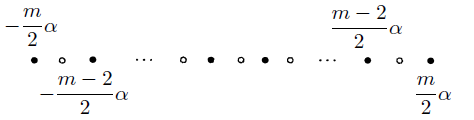
\includegraphics[width=8cm, height =2cm]{weightsl2.png}
\end{align}
Note that we can already distinguish the representations of $\mf{sl}(2,\bb{C})$ by looking at the ends of the weight diagram - $\frac{m}{2}\alpha$ or $-\frac{m}{2}\alpha$. This kind of phenomenon will carry over to all semisimple Lie algebra representations. However, in the more general case, the rank $\dim \mf{h}^*$ is higher than 1 and the distribution of weights on $\mf{h}^*$ will not be a straight line as in the rank one case.\\
Yet the weight distribution in the general case follows a pattern: There is a symmetry on the spots containing the weights of an irreducible representation, like this example showing in Hall p.151:
$$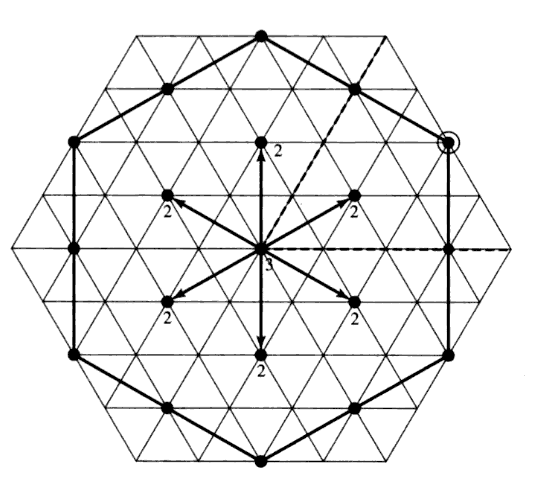
\includegraphics[width=8cm, height =6cm]{weight.png}$$
The example shows the weight of an irreducible representation in $\mf{sl}(3,\bb{C})$ and the plane is $\mf{h}^*$ which is 2-dimensional. One can see there is a symmetry on the distribution of weights (in the $\mf{sl}(2,\bb{C})$ example, the symmetry is preisely flipping over the weights along the origin.)\\
With this symmetry, one can determine the irreducible representation by looking at the `corners' of the weight diagram. This is precisely the circled dot on the diagram above (or the end $\frac{m}{2}\alpha$ in the $\mf{sl}(2,\bb{C})$ example).\\
This will be the next topic we are to study next Sections: all the weight diagrams has a \textbf{Weyl group} symmetry. By fixing a \textbf{Weyl chamber}, there is only one \textbf{highest weight} (corner) on each Weyl chamber. The highest weight determines all irreducible representations of $\mf{g}$.
\section{Weyl Group}
\begin{definition}
Let $\mf{g}$ be a complex semisimple Lie algebra, and $\mf{h} = \mf{t} + i\mf{t}$ be a CSA of $\mf{g}$. Then the \textbf{Weyl group} is defined as
$$W := N_K(\mf{t})/Z_K(\mf{t})$$
where $N_K(\mf{t})$ means the normalizer of $\mf{t}$, and $Z_K(\mf{t})$ is the centralizer of $\mf{t}$.
\end{definition}
Let $w \in W$, we can define an action on $\mf{t}$ (or extend complex linearly to $\mf{h}$) by
$$w \cdot H := Ad_g(H)$$
where $g$ is a representative on $N_K(\mf{t})$ in $W$.\\

We want the Weyl group $W$ to act on the set of weights, but the weights are in $\mf{h}^*$ instead of $\mf{h}$. We therefore need to identify elements in $\mf{h}^*$ with elements in $\mf{h}^*$ using an $Ad_K$-invariant inner product on $\mf{g} = \mf{k}_{\bb{C}}$. Such inner product $\langle, \rangle$ always exists, for instance it shows up in the proof of Proposition \ref{sscompred}. In particular, for all $\alpha \in \mf{h}^*$, we can find a unique $H^{\alpha} \in \mf{h}$ such that
$$\alpha(H) = \langle H^{\alpha},H\rangle$$
for all $H \in \mf{h}$.\\
The following proposition says that the roots are left invariant by $W$, after our identification of $\mf{h}$ and $\mf{h}^*$.
\begin{proposition}
The set $\left\{ H^{\alpha}\ \Big|\ \alpha \in R\right\}$ is invariant over the action of $W$, hence $\Lambda_R$ is invariant under the action of $W$.
\end{proposition}
\begin{proof}
(a) Suppose $\alpha \in R$. So there is an element $X \in \mf{g}_{\alpha}$ so that
$$[H,X] = \alpha(H)X = \langle H^{\alpha}, H\rangle X$$
Let $g \in N_K(\mf{t})$ be a representative of the Weyl group element $w \in W$. Then we claim that $Ad_g(X)$ is also a weight vector, with
$$[H, Ad_g(X)] = \langle Ad_g(H^{\alpha}), H \rangle Ad_g(X)$$
for all $H \in \mf{h}$. Hence $Ad_g(H^{\alpha}) = H^{\alpha'}$ for some $w\cdot \alpha := \alpha' \in R$. To see why it is so,
\begin{align*}
[H,Ad_g(X)] &= Ad_g([Ad_{g^{-1}}H, X])\\
&=Ad_g(\langle H^{\alpha}, Ad_{g^{-1}}H \rangle X)\\
&=\langle Ad_g(H^{\alpha}), H \rangle Ad_g(X)
\end{align*}
\end{proof}
In fact, the collection of coroots $H_{\alpha}$ (which is inherently in $\mf{h}$) is also invariant over $W$. Before proving this, we need the following
\begin{lemma} \label{halpha}
$$H_{\alpha} = 2\frac{H^{\alpha}}{\langle H^{\alpha}, H^{\alpha} \rangle}$$
\end{lemma}
\begin{proof}
Recall that in our proof of constructing the $\mf{sl}(2,\bb{C})$-triple, $H_{\alpha}$ lies in the one-dimensional subspace $(\ker \alpha)^{\perp}$ of $\mf{h}$.\\
Now recall our definition of $H^{\alpha}$ - Suppose $H \in \ker \alpha$, then $\langle H^{\alpha}, H \rangle = \alpha(H) = 0$, hence $H^{\alpha} \in (\ker \alpha)^{\perp}$ too.\\
Since the space is one dimensional, we write $H_{\alpha} = kH^{\alpha}$ for some constant $k$. Now
$$2 = \alpha(H_{\alpha}) = \langle H_{\alpha}, H^{\alpha} \rangle = k \langle H^{\alpha}, H^{\alpha} \rangle$$
and hence the coefficient $k$ equal to that in the Lemma.
\end{proof}

\begin{proposition}
The set of coroots $\left\{ H_{\alpha}\ \Big|\ \alpha \in R\right\}$ is invariant under the action of $W$.\\
\end{proposition}
\begin{proof}
Consider $Ad_g(H_{\alpha})$ for a representative $g$ of the Weyl group element $w \in W$. Then
\begin{align*}
Ad_g(H_{\alpha}) &= 2 \frac{Ad_g(H^{\alpha})}{\langle H^{\alpha}, H^{\alpha} \rangle}\\
&= 2\frac{H^{w\cdot \alpha}}{\langle H^{\alpha}, H^{\alpha} \rangle} \ \ \ \ \text{      by Lemma}\\
&= 2\frac{H^{w\cdot \alpha}}{\langle Ad_g(H^{\alpha}), Ad_g(H^{\alpha} \rangle)} \ \ \ \ \text{by}Ad_K \text{ invarance of inner product}\\
&= 2\frac{2H^{w\cdot \alpha}}{\langle H^{w\cdot \alpha}, H^{w \cdot \alpha} \rangle}\\
&= H_{w \cdot \alpha}
\end{align*}
\end{proof}

Now let's move to the case of weight lattices and weights of a representation.
\begin{proposition} \label{wtweyl}
(a) The weight lattice $\Lambda_W$ is invariant under the action of $W$.\\
(b) Let $(\pi,V)$ be a finite-dimensional representation of a complex semisimple Lie algebra $\mf{g}$. Then the weights of $V$ and their multiplicities are invariant under the action of $W$.\\
\end{proposition}
\begin{proof}
(a) Suppose $\mu \in \Lambda_W$, i.e. $\mu(H_{\alpha}) \in \bb{Z}$ for all roots $\alpha$. Then consider a representative of the Weyl group element $Ad_g$ with $g \in \mf{k}$. We want to show
$$Ad_g (H^{\mu}) = H^{\mu'}$$
where $\mu' \in \Lambda_W$. Now for any $\alpha \in R$,
$$\mu'(H_{\alpha}) = \langle H^{\mu'}, H_{\alpha} \rangle = \langle Ad_g (H^{\mu}), H_{\alpha} \rangle = \langle H^{\mu},  Ad_g(H_{\alpha}) \rangle = \langle H^{\mu}, H_{w\cdot \alpha} \rangle = \mu(H_{w \cdot \alpha}) \in \bb{Z}$$
hence $\mu' \in \Lambda_W$.\\
(b) Suppose $\mu \in \mf{h}^*$ is a weight of $(\pi,V)$, i.e. there is a $v \in V$ so that $\pi(H)v = \mu(H)v$ for all $h \in \mf{h}$, then suppose $g$ is an element corresponding to $w \in W$:
\begin{align*}
\pi(H) \Pi(g)v &= \Pi(g) \Pi(g^{-1})\pi(H)\Pi(g)v\\
&= \Pi(g) \pi(Ad_{g^{-1}}(H))v\\
&= \mu(Ad_{g^{-1}}(H)) \Pi(g)v\\
&= \langle H^{\mu}, Ad_{g^{-1}}(H) \rangle \Pi(g)v\\
&= \langle Ad_{g}(H^{\mu}), H \rangle \Pi(g)v\\
\end{align*}
so $\Pi(g)v$ is also a weight vector with weight $w\cdot \mu$ satisfying $H^{w \cdot \mu} = Ad_g(H^{\mu})$.
\end{proof}
This justifies our weight diagram - there is a symmetry among the weights.\\

\noindent Our next task is to look carefully how the Weyl group looks like and how it acts on $\mf{h}$ and in particular $\Lambda_W$.
\begin{theorem}
For each $\alpha \in R$, there is an element $s_{\alpha} \in W$ such that
$$s_{\alpha}H^{\alpha} = H^{-\alpha}$$
and for any $H \in \ker \alpha$,
$$s_{\alpha}H = H$$
\end{theorem}
\begin{proof}
For each root $\alpha$, take $X_{\alpha}, Y_{\alpha}, H_{\alpha}$ as an $\mf{sl}(2,\bb{C})$ triple. Recall that if we write $X_{\alpha} = X_1 + iX_2$, we can take $Y_{\alpha} = -X_1 + iX_2 \in \mf{g}_{-\alpha}$ and hence $X_{\alpha} - Y_{\alpha} = 2X_1 \in \mf{k}$. Consider
$$g_{\alpha} = e^{\pi X_1} = e^{\frac{\pi}{2}(X_{\alpha} - Y_{\alpha})} \in K$$
We claim that $g_{\alpha}$ defines an element in $N_K(\mf{t})$, and it satisfies the properties stated in the Theorem:\\
(1) Suppose $H \in \ker \alpha$, then $\alpha(H) = 0$, then
$$Ad_{g_{\alpha}}H = e^{ad_{\frac{\pi}{2}(X_{\alpha} - Y_{\alpha})}}H = H + \frac{\pi}{2}[X_{\alpha} - Y_{\alpha},H] + \frac{1}{2}(\frac{\pi}{2})^2[X_{\alpha} - Y_{\alpha},[X_{\alpha} - Y_{\alpha},H]] + \dots$$
but $[X_{\alpha},H] = -\alpha(H)X_{\alpha} = 0$ and similarly for $Y_{\alpha}$. Therefore all the non-constant term vanishes, and $Ad_{g_{\alpha}}H = H$.\\
(2) Suppose $H \in (\ker \alpha)^{\perp}$, so $H$ must be a linear multiple of $H^{\alpha}$. In particular, we can take $H = H_{\alpha}$ and get
$$Ad_{g_{\alpha}}H_{\alpha} = e^{ad_{\frac{\pi}{2}(X_{\alpha} - Y_{\alpha})}}H_{\alpha} = H_{\alpha} + \frac{\pi}{2}[X_{\alpha} - Y_{\alpha},H_{\alpha}] + \frac{1}{2}(\frac{\pi}{2})^2[X_{\alpha} - Y_{\alpha},[X_{\alpha} - Y_{\alpha},H_{\alpha}]] + \dots$$
This becomes an $\mf{sl}(2,\bb{C})$ calculation, and we will omit the details.
\end{proof}

\begin{corollary}
For any root $\alpha \in R$ and any $\beta \in \mf{h}^*$,
$$H^{s_{\alpha} \cdot \beta} := s_{\alpha}(H^{\beta}) = H^{\beta - 2\frac{ \langle H^{\alpha}, H^{\beta} \rangle}{ \langle H^{\alpha}, H^{\alpha} \rangle} \alpha} $$
\end{corollary}
\begin{proof}
For any $H^{\beta}$, the orthogonal decomposition gives
$$H^{\beta} = \frac{\langle H^{\alpha}, H^{\beta} \rangle}{ \langle H^{\alpha}, H^{\alpha} \rangle} H^{\alpha} + (H^{\beta} - \frac{\langle H^{\alpha}, H^{\beta} \rangle}{ \langle H^{\alpha}, H^{\alpha} \rangle} H^{\alpha})$$
where the first term is in $(\ker \alpha)^{\perp}$ and the second term is in $\ker \alpha$. So the above Theorem says
$$s_{\alpha}H^{\beta} = -\frac{\langle H^{\alpha}, H^{\beta} \rangle}{ \langle H^{\alpha}, H^{\alpha} \rangle} H^{\alpha} + (H^{\beta} - \frac{\langle H^{\alpha}, H^{\beta} \rangle}{ \langle H^{\alpha}, H^{\alpha} \rangle} H^{\alpha}) = H^{\beta} - 2\frac{\langle H^{\alpha}, H^{\beta} \rangle}{ \langle H^{\alpha}, H^{\alpha} \rangle} H^{\alpha}$$
as in the statement of the Corollary.
\end{proof}

\noindent Note that if $\beta \in \Lambda_W$, $\beta(H_{\alpha}) \in \bb{Z}$ for all $\alpha \in R$. However, a similar proof of Lemma \ref{halpha} says that
$$H_{\alpha} = 2\frac{H^{\alpha}}{ \langle H^{\alpha}, H^{\alpha} \rangle}$$
and hence
$$\beta(H_{\alpha}) = \langle H^{\beta}, H_{\alpha} \rangle = 2\frac{\langle H^{\alpha}, H^{\beta} \rangle}{ \langle H^{\alpha}, H^{\alpha} \rangle} \in \bb{Z}$$
Therefore,
$$s_{\alpha}H^{\beta} = H^{\beta} - 2\frac{\langle H^{\alpha}, H^{\beta} \rangle}{ \langle H^{\alpha}, H^{\alpha} \rangle} H^{\alpha}$$
with the first term in $\Lambda_W$ and the second term in $\Lambda_R \subset \Lambda_W$, hence it is also in $\Lambda_W$. Combined with the Theorem below, we obtain another proof of Proposition \ref{wtweyl}(a): (The same argument goes for $\beta \in \Lambda_R$ as well)
\begin{theorem}
The Weyl group $W$ is generated by $\left\{ s_{\alpha}\ \Big|\ \alpha \in R\right\}$.
\end{theorem}
\begin{example}
Let's look at the case of $\mf{sl}(2,\bb{C})$ before we go further. Here $R = \left\{ \alpha := \epsilon_1 - \epsilon_2 \right\} \subset \mf{h}^*$. Then the Weyl group is just generated by $s_{\alpha}$ with representative
$$g_{\alpha} = e^{\frac{\pi}{2}(X_{\alpha} - Y_{\alpha})} = e^{\left( \begin{array}{cc}
 0 & \pi/2\\
-\pi/2 & 0 \end{array} \right)} = \left( \begin{array}{cc}
 0 & 1\\
-1 & 0 \end{array} \right)$$
In this case, $\mf{h}^*$ is one-dimensional spanned by $\alpha$, and $s_{\alpha}\cdot \alpha = -\alpha$. Therefore it acts on $\Lambda_R = \bb{Z}\alpha$ and $\Lambda_W = \frac{\bb{Z}}{2}\alpha$ by flipping about the origin.\\
In particular, it flips the weights $\left\{-\frac{m}{2}\alpha,\dots,\frac{m}{2}\alpha\right\}$ appearing in $(\pi_m,V)$. This is precisely what we meant by `symmetry of weight diagram' mentioned before this Section.\\

\noindent Now let's look at the example of $\mf{sl}(3,\bb{C})$. Recall we have $R = \left\{\pm(\epsilon_1 - \epsilon_2), \pm(\epsilon_1 - \epsilon_3), \pm(\epsilon_2 - \epsilon_3)\right\}$ and $H_{\epsilon_i - \epsilon_j} = E_{ii} - E_{jj}$. Then the reflections $s_{\epsilon_1 - \epsilon_2}$ acts on the weight lattice $\beta \in \Lambda_W$ by
$$s_{\epsilon_1 - \epsilon_2} \beta = \beta - 2\frac{\langle H^{\epsilon_1 - \epsilon_2}, H^{\beta} \rangle}{\langle H^{\epsilon_1 - \epsilon_2}, H^{\epsilon_1 - \epsilon_2} \rangle} (\epsilon_1 - \epsilon_2) = \beta - \beta(H_{11} - H_{22})(\epsilon_1 - \epsilon_2)$$
For example, if $\beta = 4\epsilon_1 + 2\epsilon_2 \in \Lambda_W$, then $s_{\epsilon_1 - \epsilon_2} \beta = 2\epsilon_1 + 4\epsilon_2$. This corresponds to the reflection of the circled dot in the diagram to the dot on the top of the diagram. In fact, the reflection by $\epsilon_1 - \epsilon_2$ is given by the reflection on the slanted dotted line on the diagram.
\end{example}
\section{Simple Roots and Weyl Chamber}
As we mentioned, we need to pick one `fundamental domain' for our weight diagram, so that we can fill out the whole weight diagram from the domain using Weyl group symmetry. This is the main content of this Section.\\
The following definition is essential in picking which domain we
\begin{definition}
Let $R$ be a root system for a complex semisimple Lie group. A \textbf{base} of $R$ is a subset $\Delta = \left\{\alpha_1, \dots, \alpha_r\right\}$ of $R$ so that\\
(1) it spans the whole $\mf{h}^*$, and \\
(2) for every $\alpha \in R$
$$\alpha = \sum_i n_i \alpha_i$$
where $n_i \in \bb{Z}$ are either all $\geq 0$ or $\leq 0$.
Upon fixing such $\Delta$, the $\alpha$'s having $n_i \geq 0$ for all $i$ are called \textbf{positive roots} $R^+$, and the $\alpha$'s having $n_i \leq 0$ for all $i$ are called \textbf{negative roots} $R^-$.\\
The elements $\alpha_i \in \Delta$ is called a positive \textbf{simple root}.
\end{definition}
\begin{example}
Let $\mf{g} = \mf{sl}(n+1,\bb{C})$, then
$$R = \left\{ \epsilon_i - \epsilon_j \right\}_{1 \leq i \neq j \leq n+1}$$
then the simple roots $\Delta$ can be chosen to be
$$\Delta = \left\{ \epsilon_i - \epsilon_{i+1} \right\}_{1 \leq i \leq n}$$
Let $\mf{g} = \mf{so}(2n+1,\bb{C})$, then
$$\Delta = \left\{ \epsilon_i - \epsilon_{i+1} \right\}_{1 \leq i \leq n-1} \cup \left\{\epsilon_{n}\right\}$$
Let $\mf{g} = \mf{sp}(2n,\bb{C})$, then
$$\Delta = \left\{ \epsilon_i - \epsilon_{i+1} \right\}_{1 \leq i \leq n-1} \cup \left\{2\epsilon_{n}\right\}$$
Let $\mf{g} = \mf{so}(2n,\bb{C})$, then
$$\Delta = \left\{ \epsilon_i - \epsilon_{i+1} \right\}_{1 \leq i \leq n-1} \cup \left\{\epsilon_{n-1}+ \epsilon_n \right\}$$
\end{example}
It is not obvious that a base exists for every root system. But let us assume this for now and see how we move forward:
\begin{definition}
The set of $\mu \in i\mf{t}^* \subset \mf{h}^*$ satisfying
$$\mu(H_{\alpha}) \geq 0$$
for all positive simple roots $\alpha \in \Delta$ is called the \textbf{fundamental Weyl chamber} $\mc{W}$ relative to $\Delta$. The elements in
$$\mc{W} \cap \Lambda_W$$
are called \textbf{dominant integral elements}.
\end{definition}
Obviously, we want the elements in $$\mc{W} \cap \Lambda_W$$ generate the weight lattice $\Lambda_W$. In other words, we want to prove
\begin{lemma}
Let $\mu \in i\mf{t}^*$, then there exists an element $w \in W$ so that $w \cdot \mu \in \mc{W}$.
\end{lemma}
\begin{exercise}
Finish the above Lemma by proving the following:\\
(a)\ Let $\beta \in R^+$ be a positive root, and $\alpha \in \Delta^+$ a simple root. If $\beta \neq \alpha$, then show that
$$s_{\alpha} \cdot \beta \in R^+$$
(Hint: write $\beta$ as a sum of simple roots - $\beta = \sum_{\gamma \in \Delta^+} k_{\gamma} \gamma$ with $k_{\gamma} \in \bb{N}$.)\\
(b)\ Let $\rho = \frac{1}{2}\sum_{\alpha \in R^+} \alpha$ and $\alpha \in \Delta^+$. Show that
$$\rho(H_{\alpha}) = 1$$
and hence $\rho \in \Lambda_W$.\\
(c)\  For any $\mu \in i\mf{t}^*$, let $w \in W$ be such that $\langle w^{-1}\delta, \mu \rangle$ is as large as possible, i.e.
$$\langle w^{-1}\delta, \mu \rangle \geq \langle w^{-1}s_{\alpha}\delta, \mu \rangle$$
for all $\alpha \in \Delta^+$. Show that $\langle \alpha, mu \rangle \geq 0$.
\end{exercise}
For example, the Weyl chamber of $\mf{sl}(3,\bb{C})$ is the area bounded by the two dotted lines in the diagram.

\section{Cartan-Weyl's Highest Weight Theorem}
Here is the statement of Cartan-Weyl's classification:
\begin{theorem}
Let $\mf{g}$ be a complex semisimple Lie algebra. Then there is a one-to-one correspondence between finite-dimensional, irreducible representations of $\mf{g}$ and the dominant integral elements $\mu \in \Lambda_W \cap \mc{W}$.
\end{theorem}
There are a few intermediate steps in proving this Theorem. The basic idea is, for every irreducible representation $\pi$, we just consider the weights of $\pi$ in $\Lambda_W \cap \mc{W}$. They form the `fundamental domain' as we explored in the previous Sections. It happens that all such `fundamental domains' have the `highest' weight. Then we use the highest weight to classify all finite-dimensional irreducible representations.
\begin{definition} \label{higher}
Let $\mu_1$ and $\mu_2$ be elements in $\mf{h}^*$. Then $\mu_1$ is \textbf{higher} than $\mu_2$, or $\mu_1 \succeq \mu_2$, if there are non-negative real numbers $p_i$ such that
$$\mu_1 = \mu_2 + \sum_i p_i \alpha_i$$
with $\alpha_i \in \Delta$ for all $i$. \\
Let $(\pi,V)$ be a representation of $\mf{g}$. Then a weight $\mu_0$ is called the \textbf{highest weight} if $\mu_0 \succeq \mu$ for all weights in $\pi$.
\end{definition}
We will tackle the Theorem into the following steps:\\
(1) Every irreducible representation $\pi$ has a unique highest weight of multiplicity one, and the highest weight must be an element in $\Lambda_W \cap \mc{W}$.\\
(2) Two irreducible representations with the same highest weight must be isomorphic.\\
(3) For each element $\mu \in \Lambda_W \cap \mc{W}$, construct an irreducible representation $\pi$ with highest weight $\mu$.\\
\begin{proposition}
Let $(\pi,V)$ be an irreducible representation of $\mf{g}$. Then it must have a unique highest weight of multiplicity one.
\end{proposition}
\begin{proof}
$V$ is finite dimensional, so we have finite number of weights. Pick a highest weight $\mu_0$ in $\pi$, i.e. there are no other $\mu \succeq \mu_0$ appearing in $\pi$. Now $\mf{g}$ is spanned by elements of the form $$\left\{X_{\alpha}, Y_{\alpha}, H_{\alpha}\right\},\ \alpha \in R^+$$
(since $Y_{\alpha} \in \mf{g}_{-\alpha}$ and $H_{-\alpha} = -H_{\alpha}$). Then for the corresponding weight vector $v$,
$$\pi(X_{\alpha})v = 0$$
for all $\alpha \in R^+$, or else it is a weight vector of weight $\mu + \alpha$. Now consider the subspace $U$ spanned by elements of the form
$$\pi(Y_{\alpha_1})\dots \pi(Y_{\alpha_k})v$$
This forms an invariant subspace of $V$ - acting $\pi(Y_{\alpha})$ on $U$ obviously leaves $U$ invariant. Also, for any $H \in \mf{h}$
\begin{align*}
[\pi(H)\pi(Y_{\alpha_1})\dots \pi(Y_{\alpha_k})]v &= [\pi(Y_{\alpha_1})\pi(H)\dots \pi(Y_{\alpha_k})]v + [\pi([H,Y_{\alpha_1}])\pi(Y_{\alpha_2})\dots \pi(Y_{\alpha_k})]v\\
&= [\pi(Y_{\alpha_1})\pi(H)\dots \pi(Y_{\alpha_k})]v -2\alpha_1(H) [\pi(Y_{\alpha_1})\pi(Y_{\alpha_2})\dots \pi(Y_{\alpha_k})]v\\
&= \dots \\
&= [\pi(Y_{\alpha_1})\pi(Y_{\alpha_2}) \dots \pi(Y_{\alpha_k})\pi(H)]v - u\\
&= \mu(H)[\pi(Y_{\alpha_1})\pi(Y_{\alpha_2}) \dots \pi(Y_{\alpha_k})]v - u
\end{align*}
where $u \in U$ is the sum of the remaining terms. Hence it is invariant under $\pi(H)$. A similar argument shows that it is invariant under $\pi(X_{\alpha})$ since $\pi(X_{\alpha})v = 0$, so it is an invariant subspace of $V$, and must be equal to $V$ by irreducibility.\\
Now, each vector of $U = V$ in the above form has weight $\mu - \sum \alpha_i$, which is lower than $\mu$. So it must have the unique highest weight $\mu$. Furthermore, the only space in $U$ having weight $\mu$ is $\mathrm{Span}\left\{v\right\}$ (recall thhat weight vectors of different weights are linearly independent). So the multiplicity of the highest weight $\mu$ is one.
\end{proof}
\begin{proposition}
The highest weight $\mu$ of an irreducible representation $(\pi,V)$ must lie in the dominant weight lattice $\Lambda_W \cap \mc{W}$.
\end{proposition}
\begin{proof}
The highest weight $\mu$ and the highest weight vector $v$ has the property that $\pi(X_{\alpha})v = 0$ for all $\alpha \in R^+$. Restricting the representation to the $\mf{sl}(2,\bb{C})$-triple $\mf{s}_{\alpha}$, $v$ is like the $u_0$ vector in the $\mf{sl}(2,\bb{C})$ case, and hence for any $\alpha \in R^+$,
$$\mu(H_{\alpha}) = \pi(H_{\alpha})v = mv$$
for some non-negative integer $m$, hence $\mu \in \mc{W}$.
\end{proof}
\begin{proposition}
Let $(\pi_1,V_1)$ and $(\pi_2, V_2)$ be two irreducible representations with the same highest weight $\mu$. Then they are isomorphic.
\end{proposition}
\begin{proof}
Consider the representation $V_1 \oplus V_2$ of $\mf{g}$. Write $U$ as the smallest invariant subspace of $V_1 \oplus V_2$ containing the vector $(v_1,v_2) \in V_1 \oplus V_2$, where $v_1$ and $v_2$ are the highest weight vector in $V_1$ and $V_2$ respectively. Then $U$ is irreducible, containing the highest weight $\mu$.\\
Now consider the projection map $p_i: V_1 \oplus V_2 \to V_i$. It is obviously an intertwining map, and so are their restrictions $p_i  \Big|_U: U \to V_i$. Note that $p_i|U$ are non-zero maps by construction, and hence Schur's Lemma says $p_i  \Big|_U$ are isomorphisms. That is, $V_1 \cong U \cong V_2$.
\end{proof}

\section{Verma Modules}
To finish the Theorem of highest weight, we need to construct a finite-dimensional representation with highest weight $\mu \in \mc{W} \cap \Lambda_W$. We will realize the representation $V_{\mu}$ using \textbf{Verma modules}.
\begin{theorem}
Let $\mf{g}$ be a complex semisimple Lie algebra with positive roots $R^+ = \left\{\alpha_1, \dots, \alpha_m\right\}$. For any $\mu \in \mf{h}$, there is a representation $(M(\mu), \pi)$ of highest weight $\mu$ so that $M(\mu)$ is an infinite-dimensional vector space, with elements being a finite linear combination of vectors of the form
$$\pi(Y_{i_1})\pi(Y_{i_2})\dots \pi(Y_{i_N})v_0$$
where $Y_{i} \in \mf{g}_{-\alpha_i}$ and $v_0$ is the highest weight vector in $M(\mu)$.
\end{theorem}
\noindent Note that we do not restrict $\mu$ to be dominant and integral. Also, it only defines a representation of the Lie algebra - it does not integrate to a representation of Lie groups in general.\\
We do not give the precise proof of the Theorem, but instead give a few useful observations that leads to the Theorem:\\
(1) For all positive roots $\alpha_i \in R^+$, fix $Y_i \in \mf{g}_{-\alpha_i}$. Define $M(\mu)$ to be a vector space spanned by vectors of the form
$$Y_{i_1}\dots Y_{i_N}v_0$$
with the relations
$$Y_1Y_2v = Y_2Y_1v + \sum_l a_l Y_{i_l}v$$
where $[Y_1, Y_2] = \sum_l a_l Y_{i_l}$.\\
(2) Define $\pi(Y_i)v = Y_iv$ for any $v \in M(\mu)$. Check that it is well-defined and hence the vectors in $M(\mu)$ can be written in the form as shown in the Theorem.\\
(3) Define $\pi(H)v_0 = \mu(H)v_0$, and
$$\pi(H) \pi(Y_{i_1})\dots \pi(Y_{i_N})v_0 = (\mu - \alpha_{i_1} - \dots - \alpha_{i_N})\pi(Y_{i_1})\dots \pi(Y_{i_N})v_0 $$
(4) Define $\pi(X)v_0 = 0$ for all $X \in \mf{g}_{\alpha_i}$, and
$$\pi(X) \pi(Y_{i_1})\dots \pi(Y_{i_N})v_0 = \pi(Y_{i_1})\pi(X)\dots \pi(Y_{i_N})v_0v_0 + \pi([X,\pi(Y_{i_1})]) \dots \pi(Y_{i_N})v_0 = \dots$$
until $\pi(X)$ goes to the right.\\
(5) We need to check that the vectors $\pi(H) \pi(Y_{i_1})\dots \pi(Y_{i_N})v_0$ or $\pi(X) \pi(Y_{i_1})\dots \pi(Y_{i_N})v_0$ does not depend on how we use the commutation relations (we have been using commutation relations from left to right at (3) and (4)), e.g. if
$$\pi(Y_1)\pi(Y_2)v_0 = a_l \pi(Y_l)v_0$$
is it true that
$$\pi(H)\pi(Y_1)\pi(Y_2)v_0 = \sum_l a_l \pi(H)\pi(Y_l)v_0$$
i.e. is $\mu-\alpha_1 - \alpha_2 = \sum_l a_l (\mu - \alpha_l)$?
This can be checked by studying the \textbf{universal enveloping algebra}, which you will come across next semester.\\

\noindent Since we want a finite dimensional space, we need to take away a lot of elements in $V_{\mu}$ to make it finite dimensional. This is the space we want to get rid of:
\begin{definition}
Let $U(\mu)$ be the subspace of $M(\mu)$ so that it does not contain any component of $v_0$, and for any $u \in U(\mu)$, none of the elements
$$\pi(X_1) \dots \pi(X_n)u$$
have component of $v_0$.
\end{definition}
Then the space
$$L(\mu) := M(\mu)/U(\mu)$$
is irreducible: first of all, it is easy to check that $U(\mu)$ is an invariant subspace. Now suppose there exists $0 \neq [v] \in M(\mu)/U(\mu)$, i.e. $v \notin U(\mu)$, then there exists $\pi(X_1)\dots\pi(X_n)$ so that $\pi(X_1)\dots\pi(X_n)v$ has non-zero $v_0$ component. Write
$$u = \pi(X_1)\dots\pi(X_n)v = kv_0 + v'$$
where $v'$ is a linear combination of weight vectors of weight $\lambda \neq \mu$. Consider $u' = (\pi(H) - \lambda(H)I)u$, then the $\lambda$ weight space component in $v'$ gets killed. Keep applying this action on other weights $\lambda' \neq \mu$, and we finally kill all $v'$ and left with $kv_0$. Hence we can generate every vector in $M(\mu)$ from $v$, in particular we can generate $L(\mu)$ by $v'$, and we are done.\\

It is not clear whether $L(\mu)$ is finite-dimensional or not. In fact, what we have proved above does not require $\mu$ to be dominant integral, so we do not expect $L(\mu)$ to be finite-dimensional in general.\\
The proposition below uses the criterion of $\mu$ being dominant integral, which essential in proving the finite-dimensionality of $L(\mu)$:
\begin{proposition}
For any positive root $\alpha$, let $X_{\alpha} \in \mf{g}_{\alpha}$ and $Y_{\alpha} \in \mf{g}_{-\alpha}$. If $\mu$ is dominant integral, then for all $v \in L(\mu)$ there exists $k_v \in \bb{N}$ so that
$$\pi(X_{\alpha})^{k_v} v = \pi(Y_{\alpha})^{k_v} v = 0$$
\end{proposition}

\begin{theorem}
If $\mu$ is dominant integral, then the weight space of $L(\mu)$ is invariant over the Weyl group.\\
Consequently, $L(\mu)$ is finite dimensional.
\end{theorem}
\begin{proof}
Recall the Weyl group is generated by elements $s_{\alpha} = e^{\frac{\pi}{2}(X_{\alpha} - Y_{\alpha})} = e^{X_{\alpha}}e^{-Y_{\alpha}}e^{X_{\alpha}}$. By the last Proposition, we can define the element
$$s_{\alpha} = e^{\pi(X_{\alpha})}e^{-\pi(Y_{\alpha})}e^{\pi(X_{\alpha})}$$
acting on $L(\mu)$. Check that it maps the $\lambda$ weight space to $s_{\alpha} \cdot \lambda$ weight space.
\end{proof}

\section{Fundamental Weights and Some Explicit Constructions}
We would like to present a common way to denote the elements in the dominant weight lattice:
\begin{definition}
Let $\mf{g}$ be a complex semisimple Lie algebra, $R$ be its root space and $\Delta = \left\{ \alpha_1, \dots, \alpha_n\right\}$ be the set of positive simple roots.\\
Then the \textbf{fundamental weights} of $\mf{g}$ are the elements $\left\{ \omega_1, \dots, \omega_n \right\} \subset \mf{h}^*$ such that
$$\omega_i(H_{\alpha_j}) = \delta_{ij}$$
\end{definition}
Therefore, every $\mu \in \Lambda_W \cap \mc{W}$ in the fundamental weight lattice can be written uniquely as a linear combination of $\omega_i$'s.

\begin{example}
Let $\mf{g} = \mf{sl}(n+1,\bb{C})$, then $\Delta = \left\{\epsilon_1 - \epsilon_2, \dots, \epsilon_n - \epsilon_{n+1}\right\}$, and $H_{\epsilon_i - \epsilon_{i+1}} = E_{ii} - E_{i+1,i+1}$. So we can take
$$\omega_i = \epsilon_1 + \dots + \epsilon_i$$
\end{example}

By Cartan-Weyl classification of irreducible representations, each $\omega_i$ corresponds to an irreducible representation $(\pi_1,V_i)$. They are called the \textbf{fundamental representations} of $\mf{g}$. Here is the reason why they are called fundamental:
\begin{proposition}
Every irreducible representation $(\pi,V)$ appears as an invariant subspace of a tensor product of fundamental representations.
\end{proposition}
\begin{proof}
Suppose the irreducible representation $V$ has highest weight $\mu \in \mc{W} \cap \Lambda_W$. Then for any positive simple roots $\alpha_i$, $k_i = \mu(H_{\alpha_i}) \in \bb{N}$ and hence
$$\mu = k_1\omega_1 + \dots + k_n \omega_n$$
Now consider $V := \bigotimes_{i=1}^{n} Sym^{k_i}V_i$. Then for the (unique) highest weight vector $v_i \in V_i$, $v_i^{k_i} \in Sym^{k_i}V_i$ and $\pi(H)v_i^{k_i} = k_i\omega_i(H)v^{k_i}$. It is the unique weight vector with weight $k_i\omega_i$.\\
Also, the vector $v_1^{k_1} \otimes v_2^{k_2} \dots \otimes v_n^{k_n} \in V$ is a highest weight vector. Now completely decompose $V$ into irreducible representations, so all summands $V_{\lambda}$ of $V$ are parametrized by dominant weight $\lambda$. One of the summands must contain $V_{\mu}$ to account for the highest weight appearing in $V$.
\end{proof}
We now look at some explicit examples of fundamental representations.
\begin{example} \mbox{}\\
For $\mf{sl}(n+1,\bb{C})$, the fundamental representations are of the form $V_{\omega_i} = \wedge^i \bb{C}^{n+1}$, where $\bb{C}^{n+1}$ has the usual representation of $SL(n+1,\bb{C})$ -\\
First of all, check that the vector $v := e_1 \wedge \dots \wedge e_i \in V_{\omega_i}$ has $\pi(H)v = (\epsilon_1 + \dots + \epsilon_n)(H)v = \omega_i(H)v$. Then check that for every basis vector $v' := e_{\rho(1)} \wedge \dots \wedge e_{\rho(i)}$, we can find an element $X \in \mf{sl}(n+1,\bb{C})$ such that $\pi(X)v = v'$.\\

\noindent For $\mf{sp}(2n,\bb{C})$, recall that $\Delta = \left\{ \epsilon_1 - \epsilon_2, \dots, \epsilon_{n-1} - \epsilon_n, 2\epsilon_n\right\}$ and hence for $i =1, \dots, n$,
$$\omega_i = \epsilon_1 + \dots + \epsilon_i$$
and similarly, one can check that $\wedge^i \bb{C}^{2n}$ has a unique highest weight $\omega_i$.\\
\textbf{However, $\wedge^i \bb{C}^{2n}$ is NOT irreducible for $i > 1$.} For example, write the basis of $\bb{C}^{2n}$ by $\left\{e_1, \dots, e_n, f_1, \dots, f_n\right\}$ the vector
$$\Omega := e_1 \wedge f_1 + \dots + e_n \wedge f_n \in \wedge^2 \bb{C}^{2n}$$
(this is often called a \textbf{symplectic 2-form} of a symplectic manifold) is zero under the action of any element in $\mf{sp}(2n,\bb{C})$. So for $i > 1$, we instead consider the quotient subspace
$$V_{\omega_i} := \wedge^i \bb{C}^{2n}/\Omega \wedge (\wedge^{i-2}\bb{C}^{2n})$$
Then it is irreducible and gives the fundamental representation of $\mf{sp}(2n,\bb{C})$.\\

\noindent For $\mf{so}(2n+1,\bb{C})$, recall that $\Delta = \left\{ \epsilon_1 - \epsilon_2, \dots, \epsilon_{n-1} - \epsilon_n, \epsilon_n\right\}$ and hence for $i < n$,
$$\omega_i = \epsilon_1 + \dots + \epsilon_i\ \ ,\ \ \omega_n = \frac{1}{2}(\epsilon_1 + \dots + \epsilon_n)$$
One can check that for $i < n$, $V_{\omega_i} = \bigwedge^i \bb{C}^{2n+1}$. However, the construction of $V_{\omega_n}$ is much more complicated - this lies in the fact that $SO(2n+1,\bb{C})$ is not simply connected, and has a double universal cover $Spin(2n+1,\bb{C})$. The fundamental representation $V_{\omega_n}$ is going to be a representation of $Spin(2n+1,\bb{C})$, not $SO(2n+1,\bb{C})$.\\

\noindent For $\mf{so}(2n,\bb{C})$, recall that $\Delta = \left\{ \epsilon_1 - \epsilon_2, \dots, \epsilon_{n-1} - \epsilon_n, \epsilon_{n-1}+ \epsilon_n\right\}$ and hence for $i < n-1$,
$$\omega_i = \epsilon_1 + \dots \epsilon_i$$
and
$$\omega_{n-1} = \frac{1}{2}(\epsilon_1 + \dots \epsilon_{n-1} - \epsilon_n)\ \ ,\ \ \omega_{n} = \frac{1}{2}(\epsilon_1 + \dots \epsilon_{n-1} + \epsilon_n)$$
Similarly, $V_{n-1}$ and $V_n$ are realized as representations of $Spin(2n,\bb{C})$.
\end{example}

\section{Weight Lattice, Root Lattice and Fundamental Group}
Before we take off, it is a good idea to give a brief conclusion on the stuffs we went over in the previous Sections: We have\\

\noindent Representations of compact group $K$ $\longleftrightarrow$ Representation of compact Lie algebra $\mf{k}$ $\longleftrightarrow$ Representation of semisimple Lie algebra $\mf{g} = \mf{k}_{\bb{C}}$\\

\noindent Then we use some properties of compact groups, e.g. existence of an $Ad_K$ invariant inner product $\langle, \rangle$ to see there is a root space decomposition on $\mf{g}$ and have a root system $R$ (though we do not prove it, but the properties of $R$, e.g. $\alpha(H_{\beta}) \in \bb{Z}$ give a classification of all possible semisimple Lie algebras $\mf{g}$). Afterwards, we classify irreducible representations of $\mf{g}$.\\

\noindent The problem is to make sense out of the two $\longleftrightarrow$'s on the top - we know the $\rightarrow$ easily. For the second $\leftarrow$, we now know the classification of $\mf{g}$ and its representations, but how do we find out the compact form $\mf{k}$ from $\mf{g}$? We wrote down the compact form explicitly for the Types $A, B, C, D$, and for the exceptional $\mf{g}$, we need to use the \textit{Killing form} to determine which element in $\mf{g}$ is in $\mf{k}$. This can be done without much difficulty.\\

\noindent The problem lies in the first $\leftarrow$. We know that if $K$ is simply connected, then there is a one-to-one correspondence between Lie algebra and Lie group representations. Even better, the map $exp: \mf{k} \to K$ is surjective, so by
$$\Pi(\exp(X)) = \exp(\pi(X))$$
we know exactly how each $\Pi(k)$ looks like. But how about if $K$ is not simply connected? Recall that in computing the representations of $SU(2)$ and $SO(3,\bb{R})$ last Chapter. Since $SO(3,\bb{R})$ is not simply connected, not all irreducible representations of $\mf{so}(3,\bb{R})$ exponentiate to group level. More precisely, only half of them do exponentiate to a group representation.\\
\begin{theorem}
There is a one-to-one correspondence between connected compact Lie groups $K$ with Lie algebra $\mf{k}$, and lattices $\Lambda$ lying between $\Lambda_R$ and $\Lambda_W$,
$$\Lambda_R \subset \Lambda \subset \Lambda_W$$
The correspondence is given by the following: Given $K$, $\Lambda$ is given by the dual of
$$\Gamma := \left\{ X \in i \mf{t}\ \Big|\ exp_K(2\pi iX) = I\right\}$$
\end{theorem}
To see so, consider
$$\Gamma_W := \left\{X \in \mf{h}\ \Big|\ \alpha(X) \in \bb{Z}\ \text{for all } \alpha \in R\right\} \subset i\mf{t}$$
$$\Gamma_R := \bb{Z}\left\{H_{\alpha}\ \Big|\ \alpha \in R\right\} \subset i\mf{t}$$
Then we have a perfect pairing
\begin{align*}
\Gamma_W/\Gamma_R \times \Lambda_W/\Lambda_R &\to \bb{Q}/\bb{Z}\\
(X, \alpha) &\mapsto \alpha(X)
\end{align*}
\begin{lemma}
For any connected $G$,
$$\Gamma_R \subset \Gamma \subset \Gamma_W$$
\end{lemma}
\begin{proof}
For each $\alpha \in R$, consider the Lie algebra homomorphism $\phi: \mf{su}(2) \to \mf{g}$ by
$$\left( \begin{array}{cc}
i & 0  \\
0 & -i  \end{array} \right) \mapsto i H_{\alpha}, \left( \begin{array}{cc}
0 & 1/2  \\
-1/2 & 0  \end{array} \right) \mapsto 1/2(X_{\alpha} - Y_{\alpha}),  \left( \begin{array}{cc}
0 & i/2  \\
i/2 & 0  \end{array} \right) \mapsto i/2(X_{\alpha} + Y_{\alpha})$$
By using the Killing form, it can be checked that $i H_{\alpha}, 1/2(X_{\alpha} - Y_{\alpha}), i/2(X_{\alpha} + Y_{\alpha}) \in \mf{k}$.\\
Since $SU(2)$ is simply connected, this gets exponentiated to $\Phi: SU(2) \to K$. Therefore,
$$exp_K (2\pi iH_{\alpha}) = exp_K (2\pi \phi \left( \begin{array}{cc}
i & 0  \\
0 & -i  \end{array} \right)) = \Phi (exp_{SU(2)} \left( \begin{array}{cc}
2\pi i & 0  \\
0 & -2\pi i  \end{array} \right)) = \Phi(I) = I$$
Hence $H_{\alpha} \in \Gamma$ and we have the first inclusion.\\

For the second inclusion, suppose $X \in \Gamma$, i.e. $exp_K(2\pi iX) = I$, then for any $Z \in \mf{k}$,
$$Z = Ad(exp_K(2\pi i X))Z = \exp(ad_{2\pi i X})Z$$
in particular, if $Z = X_{\alpha} - Y_{\alpha} \in \mf{k}$, then
$$X_{\alpha} - Y_{\alpha} = Z = \exp(ad_{2\pi i X})Z = e^{2\pi i \alpha(X)}X_{\alpha} - e^{-2\pi i \alpha(X)}Y_{\alpha}$$
Since $X_{\alpha}$ and $Y_{\alpha}$ are linearly independent, this forces $\alpha(X) \in \bb{Z}$ for all $\alpha \in R$.
\end{proof}

To see its relations with fundamental group, we note the following
\begin{proposition}
Let $T := \exp(\mf{t})$ and $i: T \hookrightarrow K$ be the inclusion map. Then we have an surjection $i_*: \pi_1(T) \to \pi_1(K)$ on fundamental groups. \\
More precisely, all loops in $\pi_1(H)$ are represented by
$$t \mapsto exp_K(2\pi it X)$$
for $X \in \Gamma$, and is contractible in $G$ precisely when $X$ is an element in $\Lambda_R$. Consequently
$$\pi_1(K) \cong \Gamma/\Gamma_R$$
\end{proposition}
\begin{proof}
We give a sketch proof here since we do not go deep into algebraic topology in this course.
\end{proof}

\begin{corollary}
Let $K$ be a connected compact Lie group, then $\pi(K)$ is finite.
\end{corollary}
\begin{proof}
By the above Proposition, we only need to prove $|\Gamma/\Gamma_R|$ is finite. This in turn is equal to $|\Lambda_W/\Lambda| \leq |\Lambda_W/\Lambda_R|$. We will see the latter value is finite.\\
For any compact $K$, consider its corresponding semisimple Lie algebra $\mf{g} = \mf{k}_{\bb{C}}$. Then $\mf{g}$ is a direct sum of simple root systems. For each simple root system, introduce the \textbf{Cartan matrix} $M$ as follows: pick a positive simple roots $\left\{\alpha_1,\dots,\alpha_n\right\}$ for $\mf{g} = \mf{k}_{\bb{C}}$, then the $i,j$-entry of $M$ is given by
$$ M_{ij} = \alpha_i(H_{\alpha_j}) = 2 \frac{ \langle H^{\alpha_i}, H^{\alpha_j} \rangle}{\langle H^{\alpha_j}, H^{\alpha_j} \rangle}$$
the $|\Lambda_W/\Lambda_R|$ is equal to the product of all $\det M$'s.
\end{proof}
\begin{exercise}
Complete the above proof by showing that if $\mf{g}$ is simple, then $|\Lambda_W/\Lambda_R|$ is equal to the determinant of the Cartan matrix.
(Hint: For each $\alpha_i \in \Delta$, write $\alpha_i = \sum_j k_{ij}\omega_j$ where $\omega_j$ are fundamental weights. Then $|\Lambda_W/\Lambda_R| = \\det(k_{ij})$)
\end{exercise}


\begin{lemma}
Let $K$ be a connected compact Lie group with complex semisimple Lie algebra $\mf{k}$. Then
$$exp_K(2\pi i \Gamma_W) = Z(K)$$
Therefore, $Z(K) \cong \Gamma_W/\Gamma$.
\end{lemma}
\begin{proof}
It is easy to see that $exp_K(2 \pi i \Gamma_W) \in Z(K)$ - suppose $X$ in $\Gamma_W$, then by some similar arguments as above, $Ad(exp_K(2 \pi i X)) = e^{ad_{2\pi i X}}$ acts trivially on $\mf{k}$. Now for every element $k \in K$, $k = \exp(Y)$ by connectedness of $K$. Hence
$$Ad(exp_K(2\pi i X))k = Ad(exp_K(2\pi i X))\exp(Y) =  \exp(Ad(exp_K(2 \pi i X))Y) = \exp(Y) = k$$
and hence $exp_K(2 \pi iX) \in Z(K)$.\\
On the other direction, we need to show that every $z \in Z(K)$ must be of the form $z = \exp(X)$ for some $X \in \mf{t}$. But this is obvious since $z$ commutes with every element in the maximal torus $T$, hence it must be in $T = \exp(\mf{t})$.
\end{proof}

We are now in the position to prove the Theorem: For all compact connected Lie algebra $\mf{k}$, find a simply connected $\tilde{K}$ with Lie algebra equal to $\mf{k}$. This can be done because of Lie's Theorems (Theorem \ref{lietheorem}). Then all connected Lie groups $K$ with Lie algebra $\mf{k}$ must be isomorphic to $\tilde{K}/C$, where $C$ is a subgroup of the center of $\tilde{K}$, $Z(\tilde{K})$. In particular, if $K \cong \tilde{K}/C, \pi_1(K) \cong C \cong \Gamma/\Gamma_R$.\\
In particular,\\
- If $\tilde{K}$ is simply connected, then $C = 1$ and $\Gamma = \Gamma_R$ and $\tilde{K} \leftrightarrow \Lambda_W$ by the pairing.\\
- If $K = \tilde{K}/Z(\tilde{K})$ is \textbf{adjoint}, then $C = Z(\tilde{K})$ and $\Gamma = \Gamma_W$ and $K \leftrightarrow \Lambda_R$ by the pairing.\\

Before we go forward, let's recall the example of the double covering $SU(2) \to SO(3,\bb{R})$. We know $SU(2)$ is simply connected and $Z(SU(2)) = \left\{\pm I\right\}$, so $SO(3,\bb{R})$ is adjoint.\\

\noindent - In $SU(2)$, $X = \left( \begin{array}{cc}
p & 0  \\
0 & -p  \end{array} \right) \in \Gamma$ iff $p \in \bb{Z}$, i.e. $\Gamma = \bb{Z}{H_{\alpha}} = \Gamma_R$.\\

\noindent - In $SO(3)$, under the isomorphism of Lie algebras $\left( \begin{array}{cc}
p & 0  \\
0 & -p  \end{array} \right) \mapsto \left( \begin{array}{ccc}
0 & 0 & 0 \\
0 & 0 & -2p \\
0 & 2p & 0  \end{array} \right)$. So $X \in \Gamma$ iff
$$\exp(2\pi i \left( \begin{array}{ccc}
0 & 0 & 0 \\
0 & 0 & -2p \\
0 & 2p & 0  \end{array} \right)) = \left( \begin{array}{ccc}
1 & 0 & 0 \\
0 & \cos(4\pi p) & -\sin(4\pi p) \\
0 & \sin(4 \pi p) & \cos(4\pi p)  \end{array} \right) = I$$
i.e. $p \in \frac{1}{2}\bb{Z}$, i.e. $\Gamma = \Gamma_W$.\\

\begin{corollary}
Let $\lambda \in \Lambda_W$ be a dominant weight. Then $V_{\lambda}$ defines an irreducible representation of $K$ iff $\lambda \in \Lambda$ with $\Lambda$ specified in the Theorem.
\end{corollary}
\begin{proof}
We know that $(\pi,V_{\lambda})$ gives a representation of the simply connected cover $\tilde{K}$. To check the Corollary, let $K \cong \tilde{K}/C$ where $C \leq Z(\tilde{K})$. Then the representation $(\pi,V_{\lambda})$ descends to $K$ iff $\pi(C)$ acts trivially on $V_{\lambda}$. We have seen that $C \cong \Gamma_W/\Gamma$ and the isomorphism is given by $e_K$.\\
Take an representative $X \in \Gamma_W/\Gamma \cong C$, then $(\pi,V_{\lambda})$ is a representation of $K$ iff for all such representatives $X$,
$$\pi(e^{2\pi i X})v = v\ \text{ for all } v \in V_{\lambda}$$
Since $e^{2\pi i X} \in C \subset Z(\tilde{G})$, it is equivalent to checking the above equation with $v$ to be a highest weight vector. In this case, we need $e^{2\pi i \lambda(X)}v = v$, i.e.
$$ \lambda(X) \in \bb{Z}$$
for all representatives $X \in \Gamma/\Gamma_R$. Hence the perfect pairing says $\lambda \in \Lambda \subset \Lambda_W$ and we are done.
\end{proof}


\begin{thebibliography}{30}

\bibitem{Hall}
Brian Hall,
\emph{Lie Groups, Lie Algebras, and Representations An Elementary Introduction}

\bibitem{Lee}
John M. Lee,
\emph{Introduction to Smooth Manifolds}

\bibitem{FH}
William Fulton and Joe Harris,
\emph{Representation Theory A First Course}

\bibitem{DK}
J.J. Duistermaat and J.A.C. Kolk,
\emph{Lie Groups}

\bibitem{BtD}
Theodor Broecker and Tammo tom Dieck,
\emph{Representations of Compact Lie Groups}


\end{thebibliography}
\end{document} 